\chapter{Experiments and Results}
\section{Scalability Experiments}
This study aims to demonstrate scalability. When more servers are added, the timeliness of the simulation improves and more objects may be supported. The performance measure of interest is the maximum frame time of a server as this indicates if the simulation can be maintained when object numbers increase (keeping a low frame-time is the goal). Therefore, an injection rate is used, that spawns moving objects into the simulation as time passes.

Experiments were performed on two layouts of servers: column layout and corner layout. The column layout experiment was performed using an increasing number of servers from 1 to 10. The regions were laid out in a column configuration as shown in Fig. \ref{ColumnLayout}. Objects are injected at a constant rate, both near and far from boundaries. Injected objects are randomly selected from the following types: sphere (radius: $0.3m$), cuboid ($0.3m\mathord{\times}0.3m\mathord{\times}1.0m$) and capsule (radius: $0.3m$, height: $2m$) and start with a random velocity from the uniform distribution of: $(-10\mathord{<}x\mathord{<}10,-10\mathord{<}y\mathord{<}0,-10\mathord{<}z\mathord{<}10)m\mathord{\cdot}s^{-1}$. $50\%$ of objects are injected in a volume of $20m\mathord{\times}20m\mathord{\times}150m$ centred $12m$ away from a boundary and $15m$ above the ground plane. $50\%$ of objects are injected in the centre of a server's region in a volume of $20m\mathord{\times}20m\mathord{\times}20m$, $15m$ above the ground plane.

\definecolor{rvwvcq}{rgb}{0.08235294117647059,0.396078431372549,0.7529411764705882}
\definecolor{sim}{rgb}{0,0.2,0.5}
\begin{figure}[!t]	\begin{tikzpicture}[line cap=round,line join=round,>=triangle 45,x=1cm,y=1cm,scale=1.5]
		\clip(-2.25,0) rectangle (8.4,3.75);
	\fill[line width=0.8pt,color=rvwvcq,fill=rvwvcq,fill opacity=0.10000000149011612] (-0.02,2.5) -- (-0.02,0.5) -- (-0.22,0.5) -- (-0.22,2.5) -- cycle;
	\fill[line width=0.8pt,color=rvwvcq,fill=rvwvcq,fill opacity=0.10000000149011612] (0.22,2.5) -- (0.22,0.5) -- (0.02,0.5) -- (0.02,2.5) -- cycle;
	\fill[line width=0.8pt,color=rvwvcq,fill=rvwvcq,fill opacity=0.10000000149011612] (2.98,2.5) -- (2.98,0.5) -- (2.78,0.5) -- (2.78,2.5) -- cycle;
	\fill[line width=0.8pt,color=rvwvcq,fill=rvwvcq,fill opacity=0.10000000149011612] (3.22,2.5) -- (3.22,0.5) -- (3.022,0.5) -- (3.022,2.5) -- cycle;
	\fill[line width=0.8pt,color=rvwvcq,fill=rvwvcq,fill opacity=0.10000000149011612] (5.98,2.5) -- (5.98,0.5) -- (5.78,0.5) -- (5.78,2.5) -- cycle;
	\fill[line width=0.8pt,color=rvwvcq,fill=rvwvcq,fill opacity=0.10000000149011612] (6.222,2.5) -- (6.222,0.5) -- (6.022,0.5) -- (6.022,2.5) -- cycle;
	\fill[line width=0.8pt,color=rvwvcq,fill=rvwvcq,fill opacity=0.10000000149011612] (-1.4,1.6) -- (-1.4,1.4) -- (-1.6,1.4) -- (-1.6,1.6) -- cycle;
	\fill[line width=0.8pt,color=rvwvcq,fill=rvwvcq,fill opacity=0.10000000149011612] (1.6,1.63) -- (1.6,1.4) -- (1.4,1.4) -- (1.4,1.6) -- cycle;
	\fill[line width=0.8pt,color=rvwvcq,fill=rvwvcq,fill opacity=0.10000000149011612] (4.6,1.6) -- (4.6,1.4) -- (4.4,1.4) -- (4.4,1.6) -- cycle;
	\fill[line width=0.8pt,color=rvwvcq,fill=rvwvcq,fill opacity=0.10000000149011612] (7.6,1.6) -- (7.6,1.4) -- (7.4,1.4) -- (7.4,1.6) -- cycle;
	\fill[line width=0.8pt,color=sim,fill=sim,fill opacity=0.1] (-2.25,3) -- (-2.25,0) -- (8.25,0) -- (8.25,3) -- cycle;
	\draw [line width=0.8pt,color=rvwvcq] (-0.02,2.5)-- (-0.02,0.5);
	\draw [line width=0.8pt,color=rvwvcq] (-0.02,0.5)-- (-0.22,0.5);
	\draw [line width=0.8pt,color=rvwvcq] (-0.22,0.5)-- (-0.22,2.5);
	\draw [line width=0.8pt,color=rvwvcq] (-0.22,2.5)-- (-0.02,2.5);
	\draw [line width=0.8pt,color=rvwvcq] (0.22,2.5)-- (0.22,0.5);
	\draw [line width=0.8pt,color=rvwvcq] (0.22,0.5)-- (0.02,0.5);
	\draw [line width=0.8pt,color=rvwvcq] (0.02,0.5)-- (0.02,2.5);
	\draw [line width=0.8pt,color=rvwvcq] (0.02,2.5)-- (0.22,2.5);
	\draw (-1.5,3.5) node[anchor=center] {Server 0};
	\draw (1.5,3.5) node[anchor=center] {Server 1};
	\draw (4.5,3.5) node[anchor=center] {\textbf{...}};
	\draw (7.5,3.5) node[anchor=center] {Server N-1};
	\draw [line width=2pt] (0,0)-- (0,3);
	\draw [line width=2pt] (3,0)-- (3,3);
	\draw [line width=0.8pt,color=rvwvcq] (2.98,2.5)-- (2.98,0.5);
	\draw [line width=0.8pt,color=rvwvcq] (2.98,0.5)-- (2.78,0.5);
	\draw [line width=0.8pt,color=rvwvcq] (2.78,0.5)-- (2.78,2.5);
	\draw [line width=0.8pt,color=rvwvcq] (2.78,2.5)-- (2.98,2.5);
	\draw [line width=0.8pt,color=rvwvcq] (3.22,2.5)-- (3.22,0.5);
	\draw [line width=0.8pt,color=rvwvcq] (3.22,0.5)-- (3.022,0.5);
	\draw [line width=0.8pt,color=rvwvcq] (3.022,0.5)-- (3.022,2.5);
	\draw [line width=0.8pt,color=rvwvcq] (3.022,2.5)-- (3.22,2.5);
	\draw [line width=2pt] (6,0)-- (6,3);
	\draw [line width=0.8pt,color=rvwvcq] (5.98,2.5)-- (5.98,0.5);
	\draw [line width=0.8pt,color=rvwvcq] (5.98,0.5)-- (5.78,0.5);
	\draw [line width=0.8pt,color=rvwvcq] (5.78,0.5)-- (5.78,2.5);
	\draw [line width=0.8pt,color=rvwvcq] (5.78,2.5)-- (5.98,2.5);
	\draw [line width=0.8pt,color=rvwvcq] (6.222,2.5)-- (6.222,0.5);
	\draw [line width=0.8pt,color=rvwvcq] (6.222,0.5)-- (6.022,0.5);
	\draw [line width=0.8pt,color=rvwvcq] (6.022,0.5)-- (6.022,2.5);
	\draw [line width=0.8pt,color=rvwvcq] (6.022,2.5)-- (6.222,2.5);
	\draw [line width=0.8pt,color=rvwvcq] (-1.4,1.6)-- (-1.4,1.4);
	\draw [line width=0.8pt,color=rvwvcq] (-1.4,1.4)-- (-1.6,1.4);
	\draw [line width=0.8pt,color=rvwvcq] (-1.6,1.4)-- (-1.6,1.6);
	\draw [line width=0.8pt,color=rvwvcq] (-1.6,1.6)-- (-1.4,1.6);
	\draw [line width=0.8pt,color=rvwvcq] (1.6,1.6)-- (1.6,1.4);
	\draw [line width=0.8pt,color=rvwvcq] (1.6,1.4)-- (1.4,1.4);
	\draw [line width=0.8pt,color=rvwvcq] (1.4,1.4)-- (1.4,1.6);
	\draw [line width=0.8pt,color=rvwvcq] (1.4,1.6)-- (1.6,1.6);
	\draw [line width=0.8pt,color=rvwvcq] (4.6,1.6)-- (4.6,1.4);
	\draw [line width=0.8pt,color=rvwvcq] (4.6,1.4)-- (4.4,1.4);
	\draw [line width=0.8pt,color=rvwvcq] (4.4,1.4)-- (4.4,1.6);
	\draw [line width=0.8pt,color=rvwvcq] (4.4,1.6)-- (4.6,1.6);
	\draw [line width=0.8pt,color=rvwvcq] (7.6,1.6)-- (7.6,1.4);
	\draw [line width=0.8pt,color=rvwvcq] (7.6,1.4)-- (7.4,1.4);
	\draw [line width=0.8pt,color=rvwvcq] (7.4,1.4)-- (7.4,1.6);
	\draw [line width=0.8pt,color=rvwvcq] (7.4,1.6)-- (7.6,1.6);
	\end{tikzpicture}
\centering
\begin{tikzpicture}[line cap=round,line join=round,>=triangle 45,x=1cm,y=1cm]
		\clip(-7,0.575) rectangle (7,0.9);
\fill[line width=0.8pt,color=rvwvcq,fill=rvwvcq,fill opacity=0.1] (-2.5,0.8) -- (-2.3,0.8) -- (-2.3,0.6) -- (-2.5,0.6) -- cycle;
\draw [line width=0.8pt,color=rvwvcq] (-2.5,0.8)-- (-2.3,0.8);
\draw [line width=0.8pt,color=rvwvcq] (-2.3,0.8)-- (-2.3,0.6);
\draw [line width=0.8pt,color=rvwvcq] (-2.3,0.6)-- (-2.5,0.6);
\draw [line width=0.8pt,color=rvwvcq] (-2.5,0.6)-- (-2.5,0.8);
\draw (-2.1,0.7) node[anchor=west] {Injection Volume};

\draw [line width=2pt] (-6.5,0.7)-- (-6.3,0.7);
\draw (-6.1,0.7) node[anchor=west] {Region Boundary};
\end{tikzpicture}
\caption{Column Layout}
\label{ColumnLayout}
\end{figure}

The experiments were run for 60 seconds with an injection rate of 160 objects per second. For all experiments, a speed tolerance of $32m\mathord{\cdot}s^{-1}$ was used, which was the maximum expected speed for any object (based on maximum injection height and velocity, and gravity). The latency tolerance for these experiments was set to $2ms$ (based off measurements of latency between servers) and frame-time tolerance was set to $15ms$ (based off preliminary performance results). A time of $16ms$ was used for the physics time-step. Each experiment was repeated 50 times at various times of day to account for differing performance in cloud resources at different times. For each iteration, the maximum frame time of any server was aggregated for each $5s$ period. The mean of the aggregated maximum frame times of the iterations was then calculated and plotted.

Experiments were conducted using AWS G2.2xlarge servers located within the same geographical region. A G2.2xlarge instance uses a 2.60GHz Intel Xeon E5-2670 CPU with 16GB RAM and an NVIDIA GRID K520 (Kepler) GPU running Amazon Linux AMI 2017.09.

Fig. \ref{fig_PerCol} shows the performance of our system with rising server numbers from 1 to 10. The graph clearly shows that the addition of servers lowers the frame time throughout the experiment. This is increasingly noticeable later in the simulation when a greater number of objects are present. For higher server numbers the reduction in maximum frame time is less than for lower numbers, which is as expected as in the ideal case the workload per server would be $1/n$ of the total workload, where $n$ is the number of servers. 

From these observations it may be declared that this system is scalable in column configuration as the addition of servers results in increased performance.

\begin{figure}[!t]
	\centering
	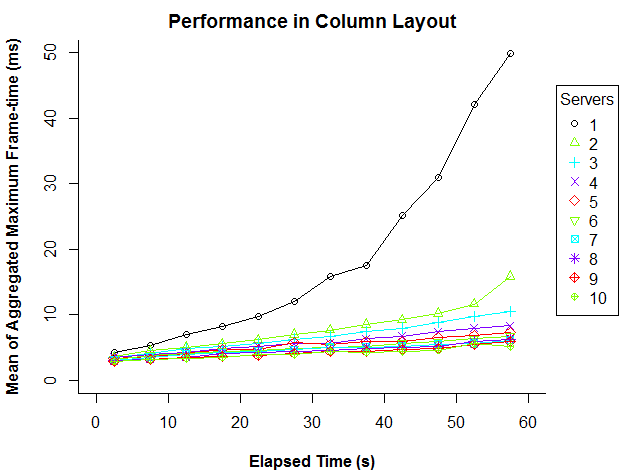
\includegraphics[width=\textwidth]{ColPerformance}
	\caption{Performance of increasing numbers of servers with an accumulating number of objects (in column layout)}
	\label{fig_PerCol}
\end{figure}

Experiments were also carried out using servers in a corner layout. The layouts of 3 and 4 servers are shown in Fig. \ref{ServerCorner}, in which the 4 server case is a 2x2 grid with a single corner intersection in the centre. The 9 server case is a 3x3 grid with 4 corner intersections. Injection rates and volume dimensions remain the same as in the column based experiments. Fig. \ref{fig_PerCor} shows the graph describing performance. The graph demonstrates that increasing the number of servers lowers the frame time. The additional processing overhead of exchanging more messages with more neighbouring servers in the 9 server experiment is outweighed by the performance gains of additional servers.

From these observations it may be declared that this system is scalable in corner configuration as the addition of servers results in increased performance.

\begin{figure}[!t]
	\begin{subfigure}{.5\textwidth}
		\begin{tikzpicture}[line cap=round,line join=round,>=triangle 45,x=1cm,y=1cm,scale=1.2]
		%	\clip(-3,-1.5) rectangle (3,3);
		\fill[line width=0.8pt,color=rvwvcq,fill=rvwvcq,fill opacity=0.10000000149011612] (-1,-0.02) -- (1,-0.02) -- (1,-0.22) -- (-1,-0.22) -- cycle;
		\fill[line width=0.8pt,color=rvwvcq,fill=rvwvcq,fill opacity=0.10000000149011612] (-0.02,2.5) -- (-0.02,0.5) -- (-0.22,0.5) -- (-0.22,2.5) -- cycle;
		\fill[line width=0.8pt,color=rvwvcq,fill=rvwvcq,fill opacity=0.10000000149011612] (0.22,2.5) -- (0.22,0.5) -- (0.02,0.5) -- (0.02,2.5) -- cycle;
		\fill[line width=0.8pt,color=rvwvcq,fill=rvwvcq,fill opacity=0.10000000149011612] (-2.5,0.22) -- (-0.5,0.22) -- (-0.5,0.02) -- (-2.5,0.02) -- cycle;
		\fill[line width=0.8pt,color=rvwvcq,fill=rvwvcq,fill opacity=0.10000000149011612] (0.5,0.22) -- (2.5,0.22) -- (2.5,0.022) -- (0.5,0.022) -- cycle;
		\fill[line width=0.8pt,color=sim,fill=sim,fill opacity=0.1] (-3,3) -- (-3,-2) -- (3,-2) -- (3,3) -- cycle;
		\draw [line width=2pt] (-3,0)-- (3,0);
		\draw [line width=2pt] (0,3)-- (0,0);
		\draw [line width=0.8pt,color=rvwvcq] (-1,-0.02)-- (1,-0.02);
		\draw [line width=0.8pt,color=rvwvcq] (1,-0.02)-- (1,-0.22);
		\draw [line width=0.8pt,color=rvwvcq] (1,-0.22)-- (-1,-0.22);
		\draw [line width=0.8pt,color=rvwvcq] (-1,-0.22)-- (-1,-0.02);
		\draw [line width=0.8pt,color=rvwvcq] (-0.02,2.5)-- (-0.02,0.5);
		\draw [line width=0.8pt,color=rvwvcq] (-0.02,0.5)-- (-0.22,0.5);
		\draw [line width=0.8pt,color=rvwvcq] (-0.22,0.5)-- (-0.22,2.5);
		\draw [line width=0.8pt,color=rvwvcq] (-0.22,2.5)-- (-0.02,2.5);
		\draw [line width=0.8pt,color=rvwvcq] (0.22,2.5)-- (0.22,0.5);
		\draw [line width=0.8pt,color=rvwvcq] (0.22,0.5)-- (0.02,0.5);
		\draw [line width=0.8pt,color=rvwvcq] (0.02,0.5)-- (0.02,2.5);
		\draw [line width=0.8pt,color=rvwvcq] (0.02,2.5)-- (0.22,2.5);
		\draw (-1.5,2.5) node[anchor=center] {Server 0};
		\draw (1.5,2.5) node[anchor=center] {Server 1};
		\draw (0,-1) node[anchor=center] {Server 2};
		\draw [line width=0.8pt,color=rvwvcq] (-2.5,0.22)-- (-0.5,0.22);
		\draw [line width=0.8pt,color=rvwvcq] (-0.5,0.22)-- (-0.5,0.02);
		\draw [line width=0.8pt,color=rvwvcq] (-0.5,0.02)-- (-2.5,0.02);
		\draw [line width=0.8pt,color=rvwvcq] (-2.5,0.02)-- (-2.5,0.22);
		\draw [line width=0.8pt,color=rvwvcq] (0.5,0.22)-- (2.5,0.22);
		\draw [line width=0.8pt,color=rvwvcq] (2.5,0.22)-- (2.5,0.022);
		\draw [line width=0.8pt,color=rvwvcq] (2.5,0.022)-- (0.5,0.022);
		\draw [line width=0.8pt,color=rvwvcq] (0.5,0.022)-- (0.5,0.22);
		\draw [line width=0.8pt,color=rvwvcq] (-1.4,1.6)-- (-1.4,1.4);
		\draw [line width=0.8pt,color=rvwvcq] (-1.4,1.4)-- (-1.6,1.4);
		\draw [line width=0.8pt,color=rvwvcq] (-1.6,1.4)-- (-1.6,1.6);
		\draw [line width=0.8pt,color=rvwvcq] (-1.6,1.6)-- (-1.4,1.6);
		\draw [line width=0.8pt,color=rvwvcq] (1.6,1.6)-- (1.6,1.4);
		\draw [line width=0.8pt,color=rvwvcq] (1.6,1.4)-- (1.4,1.4);
		\draw [line width=0.8pt,color=rvwvcq] (1.4,1.4)-- (1.4,1.6);
		\draw [line width=0.8pt,color=rvwvcq] (1.4,1.6)-- (1.6,1.6);
		
		\draw [line width=0.8pt,color=rvwvcq] (0.1,-1.6)-- (0.1,-1.4);
		\draw [line width=0.8pt,color=rvwvcq] (0.1,-1.4)-- (-0.1,-1.4);
		\draw [line width=0.8pt,color=rvwvcq] (-0.1,-1.4)-- (-0.1,-1.6);
		\draw [line width=0.8pt,color=rvwvcq] (-0.1,-1.6)-- (0.1,-1.6);
		\end{tikzpicture}
		\centering
		\begin{tikzpicture}[line cap=round,line join=round,>=triangle 45,x=1cm,y=1cm]
		%		\clip(-3.661612836111066,-0.55) rectangle (6.690195527240868,1.05);
		\fill[line width=0.8pt,color=rvwvcq,fill=rvwvcq,fill opacity=0.10000000149011612] (-2.5,0.22) -- (-2.3,0.22) -- (-2.3,0.02) -- (-2.5,0.02) -- cycle;
		\draw [line width=0.8pt,color=rvwvcq] (-2.5,0.22)-- (-2.3,0.22);
		\draw [line width=0.8pt,color=rvwvcq] (-2.3,0.22)-- (-2.3,0.02);
		\draw [line width=0.8pt,color=rvwvcq] (-2.3,0.02)-- (-2.5,0.02);
		\draw [line width=0.8pt,color=rvwvcq] (-2.5,0.02)-- (-2.5,0.22);
		\draw [line width=2pt] (-2.5,0.5)-- (-2.3,0.5);
		\draw (-2.1,0.5) node[anchor=west] {Region Boundary};
		\draw (-2.1,0.1) node[anchor=west] {Injection Volume};
		\end{tikzpicture}
		\caption{3 Server Corner Layout}
		\label{3ServerCorner}
	\end{subfigure}%
	\begin{subfigure}{.5\textwidth}
		\begin{tikzpicture}[line cap=round,line join=round,>=triangle 45,x=1cm,y=1cm,scale=1.2]
		%	\clip(-3,-3) rectangle (3,3);
		\fill[line width=0.8pt,color=rvwvcq,fill=rvwvcq,fill opacity=0.10000000149011612] (0.5,-0.02) -- (2.5,-0.02) -- (2.5,-0.22) -- (0.5,-0.22) -- cycle;
		\fill[line width=0.8pt,color=rvwvcq,fill=rvwvcq,fill opacity=0.10000000149011612] (-0.02,2.5) -- (-0.02,0.5) -- (-0.22,0.5) -- (-0.22,2.5) -- cycle;
		\fill[line width=0.8pt,color=rvwvcq,fill=rvwvcq,fill opacity=0.10000000149011612] (0.22,2.5) -- (0.22,0.5) -- (0.02,0.5) -- (0.02,2.5) -- cycle;
		\fill[line width=0.8pt,color=rvwvcq,fill=rvwvcq,fill opacity=0.10000000149011612] (-2.5,0.22) -- (-0.5,0.22) -- (-0.5,0.02) -- (-2.5,0.02) -- cycle;
		\fill[line width=0.8pt,color=rvwvcq,fill=rvwvcq,fill opacity=0.10000000149011612] (0.5,0.22) -- (2.5,0.22) -- (2.5,0.022) -- (0.5,0.022) -- cycle;
		\fill[line width=0.8pt,color=rvwvcq,fill=rvwvcq,fill opacity=0.10000000149011612] (-0.02,-0.5) -- (-0.02,-2.5) -- (-0.22,-2.5) -- (-0.22,-0.5) -- cycle;
		\fill[line width=0.8pt,color=rvwvcq,fill=rvwvcq,fill opacity=0.10000000149011612] (0.22,-0.5) -- (0.22,-2.5) -- (0.02,-2.5) -- (0.02,-0.5) -- cycle;
		\fill[line width=0.8pt,color=rvwvcq,fill=rvwvcq,fill opacity=0.10000000149011612] (-2.5,-0.022) -- (-0.5,-0.022) -- (-0.5,-0.22) -- (-2.5,-0.22) -- cycle;
		\fill[line width=0.8pt,color=sim,fill=sim,fill opacity=0.1] (-3,3) -- (-3,-3) -- (3,-3) -- (3,3) -- cycle;
		\draw [line width=2pt] (-3,0)-- (3,0);
		\draw [line width=2pt] (0,3)-- (0,0);
		\draw [line width=0.8pt,color=rvwvcq] (0.5,-0.02)-- (2.5,-0.02);
		\draw [line width=0.8pt,color=rvwvcq] (2.5,-0.02)-- (2.5,-0.22);
		\draw [line width=0.8pt,color=rvwvcq] (2.5,-0.22)-- (0.5,-0.22);
		\draw [line width=0.8pt,color=rvwvcq] (0.5,-0.22)-- (0.5,-0.02);
		\draw [line width=0.8pt,color=rvwvcq] (-0.02,2.5)-- (-0.02,0.5);
		\draw [line width=0.8pt,color=rvwvcq] (-0.02,0.5)-- (-0.22,0.5);
		\draw [line width=0.8pt,color=rvwvcq] (-0.22,0.5)-- (-0.22,2.5);
		\draw [line width=0.8pt,color=rvwvcq] (-0.22,2.5)-- (-0.02,2.5);
		\draw [line width=0.8pt,color=rvwvcq] (0.22,2.5)-- (0.22,0.5);
		\draw [line width=0.8pt,color=rvwvcq] (0.22,0.5)-- (0.02,0.5);
		\draw [line width=0.8pt,color=rvwvcq] (0.02,0.5)-- (0.02,2.5);
		\draw [line width=0.8pt,color=rvwvcq] (0.02,2.5)-- (0.22,2.5);
		\draw (-1.5,2.5) node[anchor=center] {Server 0};
		\draw (1.5,2.5) node[anchor=center] {Server 1};
		\draw (-1.5,-2.5) node[anchor=center] {Server 2};
		\draw (1.5,-2.5) node[anchor=center] {Server 3};
		\draw [line width=0.8pt,color=rvwvcq] (-2.5,0.22)-- (-0.5,0.22);
		\draw [line width=0.8pt,color=rvwvcq] (-0.5,0.22)-- (-0.5,0.02);
		\draw [line width=0.8pt,color=rvwvcq] (-0.5,0.02)-- (-2.5,0.02);
		\draw [line width=0.8pt,color=rvwvcq] (-2.5,0.02)-- (-2.5,0.22);
		\draw [line width=0.8pt,color=rvwvcq] (0.5,0.22)-- (2.5,0.22);
		\draw [line width=0.8pt,color=rvwvcq] (2.5,0.22)-- (2.5,0.022);
		\draw [line width=0.8pt,color=rvwvcq] (2.5,0.022)-- (0.5,0.022);
		\draw [line width=0.8pt,color=rvwvcq] (0.5,0.022)-- (0.5,0.22);
		\draw [line width=0.8pt,color=rvwvcq] (-0.02,-0.5)-- (-0.02,-2.5);
		\draw [line width=0.8pt,color=rvwvcq] (-0.02,-2.5)-- (-0.22,-2.5);
		\draw [line width=0.8pt,color=rvwvcq] (-0.22,-2.5)-- (-0.22,-0.5);
		\draw [line width=0.8pt,color=rvwvcq] (-0.22,-0.5)-- (-0.02,-0.5);
		\draw [line width=0.8pt,color=rvwvcq] (0.22,-0.5)-- (0.22,-2.5);
		\draw [line width=0.8pt,color=rvwvcq] (0.22,-2.5)-- (0.02,-2.5);
		\draw [line width=0.8pt,color=rvwvcq] (0.02,-2.5)-- (0.02,-0.5);
		\draw [line width=0.8pt,color=rvwvcq] (0.02,-0.5)-- (0.22,-0.5);
		\draw [line width=2pt] (0,0)-- (0,-3);
		\draw [line width=0.8pt,color=rvwvcq] (-2.5,-0.022)-- (-0.5,-0.022);
		\draw [line width=0.8pt,color=rvwvcq] (-0.5,-0.022)-- (-0.5,-0.22);
		\draw [line width=0.8pt,color=rvwvcq] (-0.5,-0.22)-- (-2.5,-0.22);
		\draw [line width=0.8pt,color=rvwvcq] (-2.5,-0.22)-- (-2.5,-0.022);
		\draw [line width=0.8pt,color=rvwvcq] (-1.4,1.6)-- (-1.4,1.4);
		\draw [line width=0.8pt,color=rvwvcq] (-1.4,1.4)-- (-1.6,1.4);
		\draw [line width=0.8pt,color=rvwvcq] (-1.6,1.4)-- (-1.6,1.6);
		\draw [line width=0.8pt,color=rvwvcq] (-1.6,1.6)-- (-1.4,1.6);
		\draw [line width=0.8pt,color=rvwvcq] (1.6,1.6)-- (1.6,1.4);
		\draw [line width=0.8pt,color=rvwvcq] (1.6,1.4)-- (1.4,1.4);
		\draw [line width=0.8pt,color=rvwvcq] (1.4,1.4)-- (1.4,1.6);
		\draw [line width=0.8pt,color=rvwvcq] (1.4,1.6)-- (1.6,1.6);
		
		\draw [line width=0.8pt,color=rvwvcq] (-1.4,-1.6)-- (-1.4,-1.4);
		\draw [line width=0.8pt,color=rvwvcq] (-1.4,-1.4)-- (-1.6,-1.4);
		\draw [line width=0.8pt,color=rvwvcq] (-1.6,-1.4)-- (-1.6,-1.6);
		\draw [line width=0.8pt,color=rvwvcq] (-1.6,-1.6)-- (-1.4,-1.6);
		\draw [line width=0.8pt,color=rvwvcq] (1.6,-1.6)-- (1.6,-1.4);
		\draw [line width=0.8pt,color=rvwvcq] (1.6,-1.4)-- (1.4,-1.4);
		\draw [line width=0.8pt,color=rvwvcq] (1.4,-1.4)-- (1.4,-1.6);
		\draw [line width=0.8pt,color=rvwvcq] (1.4,-1.6)-- (1.6,-1.6);
		\end{tikzpicture}
		\centering
		\caption{4 Server Corner Layout}
		\label{4ServerCorner}
	\end{subfigure}
\caption{Corner Layouts}
\label{ServerCorner}
\end{figure}

\begin{figure}[!t]
	\centering
	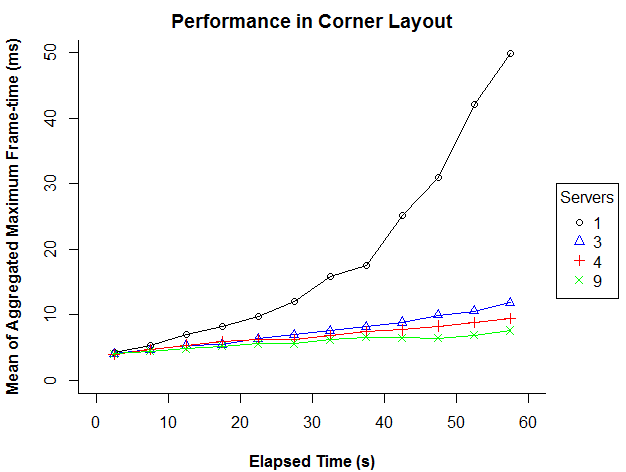
\includegraphics[width=\textwidth]{CorPerformance}
	\caption{Performance of increasing numbers of servers with an accumulating number of objects (in corner layout)}
	\label{fig_PerCor}
\end{figure}

\section{Collision Correctness Experiments}
In the following section we explore the correctness of collisions between objects, i.e. do objects have the same collision behaviour in a AP as they do in a centralised system. We are concerned with objects that are migrating and/or interacting with an object that has recently migrated.
We will now explain how a naive system can lead to erroneous collision behaviour and AP can lead to erroneous collision behaviour if speed, frame-time or latency go above the user-defined tolerances.

Erroneous collisions fall into two categories:
\begin{itemize}
	\item Missed collisions, collisions that should have taken place but were not detected by the physics engine e.g. Bullet through paper problem.
	\item Late collisions, collisions that were detected later than they should have been and result in not only different collision results, but also unstable collision response.
\end{itemize} 

%TODO: Expand on late collisions producing different results?

To understand how late collisions lead to unstable collision response, we must first understand how in real-time collision detection works. In real-time physics engines, objects move in discrete steps, as a result of this, when two objects collide, they overlap each other i.e. penetrate. The collision is resolved by calculating the forces resulting from the collision and moving the objects so they no longer overlap (in PhysX if penetration is high, the latter may be done over several physics time-steps). If the penetration is high, such as in the case of a late collision response or if two objects are moving at high speed towards one another, the collision response can no longer guarantee stable results.

It is possible to detect late collisions between objects. Given the relative speed of the two objects and the physics time-step, it possible to calculate the maximum expected penetration distance. If a collision is detected and it is above this value, it means it is a late collision.

Maximum penetration for a given speed occurs when two objects travelling directly towards each other have, in the final time-step before colliding the two objects have no distance between them, but are not overlapping, so not colliding. The next physics time-step, the collision will be detected and will have the maximum penetration possible for that relative speed. Re-arranging $s=d/t$, to $d=s.t$ and substituting the physics time-step for $t$, gives us the maximum distance (penetration) for a relative speed, and we are able to plot the maximum expected penetration line.

%In real-time physics, speed of calculation is favoured over accuracy of collision response, as a result of this 

%, this is known as the collision response (in real-time physics, speed of calculation is favoured over accuracy of collision response). High collision penetration e.g. if two objects are moving quickly towards one another, can lead to unstable collision response, which is undesirable.

%TODO: cite that deep penetration is bad

Experiments were carried out where collision results were recorded and used to detect missed and late collisions of objects. The experiment scenario used only two objects, meaning if there was a missed collision there would be no collision output. The two objects start the scenario with a specified velocity (drag and gravity are disabled), the direction being directly towards the other object and the two objects were given the same speed, which is varied throughout the experiment. Spheres were used, so rotational effects don't need to be accounted for.

\subsection{Control}

A control experiment on a centralised system was performed, in which the scenario was repeated multiple times. The purpose of this experiment was to confirm the predicted maximum expected penetration. Fig. \ref{fig_ErrorCentral} shows the penetration of objects with increasing speed in a centralised simulation and demonstrates that penetration is never greater than the maximum expected penetration.

% TODO: Add number of collisions and number of missed collisions
\begin{figure}[!t]
	\centering
	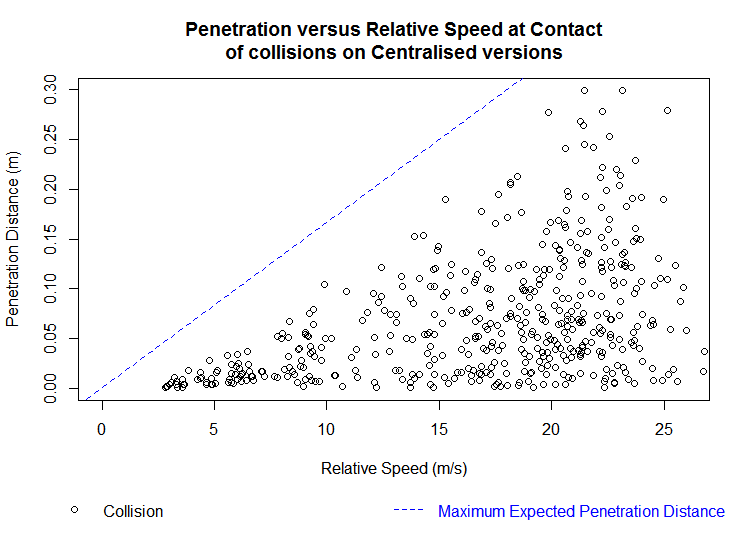
\includegraphics[width=\textwidth]{errorGraphCentral}
	\caption{Penetration of objects with increasing speed and maximum expected penetration}
	\label{fig_ErrorCentral}
\end{figure}

As relative speed increases, expected penetration increases and the erroneous penetration distance for the same aura error (aura too small or aura receive message delayed) also increases. Using Penetration time gives us a uniform error regardless of relative speed.
Re-arranging $s=d/t$, to $t=d/s$ and substituting the collision penetration for $d$ and relative speed for $s$, gives us the penetration time for a collision. It should be noted that because physics engines work in discrete time steps, this time value does not actually reflect the real time the colliding objects were penetrating each other. Correct collisions result in penetration times of up to 1 physics time step and any collision penetration times over this value are considered erroneous.

\subsection{Varying Factors}

Experiments were carried out to demonstrate the effects of varying each aura calculation factor on the correctness of collisions between objects. There are three factors that are used to determine aura size: Relative Speed; Latency; and Frame-Time. The purpose of these experiments is to demonstrate that collisions in AP are always correct if the respective values remain within their tolerances and correctness is no longer guaranteed if the tolerances are exceeded. 

In order to demonstrate the effect each factor has on collision correctness, one aura factor is varied per experiment and the other two factors are set to equal the tolerance values. For example, relative speed is varied, the latency between the servers is set to equal the latency tolerance value and the frame-time of each server is set to equal the frame-time tolerance value. The non-varied factors are set to equal the tolerance values as exceeding the tolerance value in one factor can be compensated for by having a value below the tolerance in a different factor. For example, the latency may exceed the tolerance by $5ms$, but the frame-time could be more than $5ms$ below the frame-time tolerance and the collision would still be expected to be correctly handled by AP.

Relative speed is controlled such that the two objects used in the experiment collide with each other with that relative speed. Latency is controlled using the Traffic Manager tool to emulate latency for all communications between the servers. Half of the desired latency is applied to each server, resulting in the total desired latency between servers.
Frame-time is controlled using a wait within the simulation's update loop, this is limited to a target frame-time as the resultant frame-times are a normal distribution with the target frame-time as the median. This means half of all frames are expected to be above the target frame-time, which may cause false-positives in the following experiments, however the variance in frame-time is low, so false-positives are expected to be rare.

AP can only lead to late or missed collisions when at least one object involved in the collision has just migrated (received since the last physics time-step). This is because non-migrating objects behave the same as objects in a centralised solution. In order to test this case, the same scenario as the control was used with two servers. The two spheres were given starting positions so the two would collide at a point when one of the objects is intersecting the server region boundary, thus creating the most likely situation for objects collide with each other in the first time-step after being migrated. Only objects that have just migrated are considered in the experiment results. 

The collision point of the objects has a small random variation of point along the collision axis and the collision time of the two objects is also varied by $10$ physics time-steps to prevent producing exactly the same results each iteration, but the two objects will always collide while one of the objects is intersecting the server region boundary.

The two servers use the same tolerances used in the performance experiments, a maximum speed tolerance of $32m\mathord{\cdot}s^{-1}$, maximum latency tolerance of $2ms$ and a maximum frame-time of $15ms$. Each experiment is repeated $10$ times.

For each experiment the following graphs are shown:
\begin{itemize}
	\item Collisions, plotting as points with their penetration time against the factor that is being varied along with the maximum expected penetration time and factor tolerance. This shows all the collisions that occurs and illustrates the range of penetration times that the collisions fall within as the factor is varied. %TODO: Mean penetration time
	\item Mean and Max errors against the varied factor. This includes both the mean error of all collisions, where correct collisions have an error of $0$ and the mean error of just the erroneous collisions. This illustrates how the magnitude of errors change as the factor is varied.
	\item Ratio of outliers to correct collisions and ratio of misses to total collisions against the varied factor. This illustrates how the number of errors and misses changes as the factor is varied.
\end{itemize}

%TODO: Also mention very small tolerance for detecting errors, so collisions very close to the line aren't counted as errors. Have to account for floating-point errors throughout the results process.

\subsubsection{Varying Relative Speed}

In this experiment the relative speed of the two objects being varied from $2m\mathord{\cdot}s^{-1}$ to double tolerance, $128m\mathord{\cdot}s^{-1}$ in increments of $2m\mathord{\cdot}s^{-1}$ and repeated $10$ times.

\begin{figure}
	\centering
	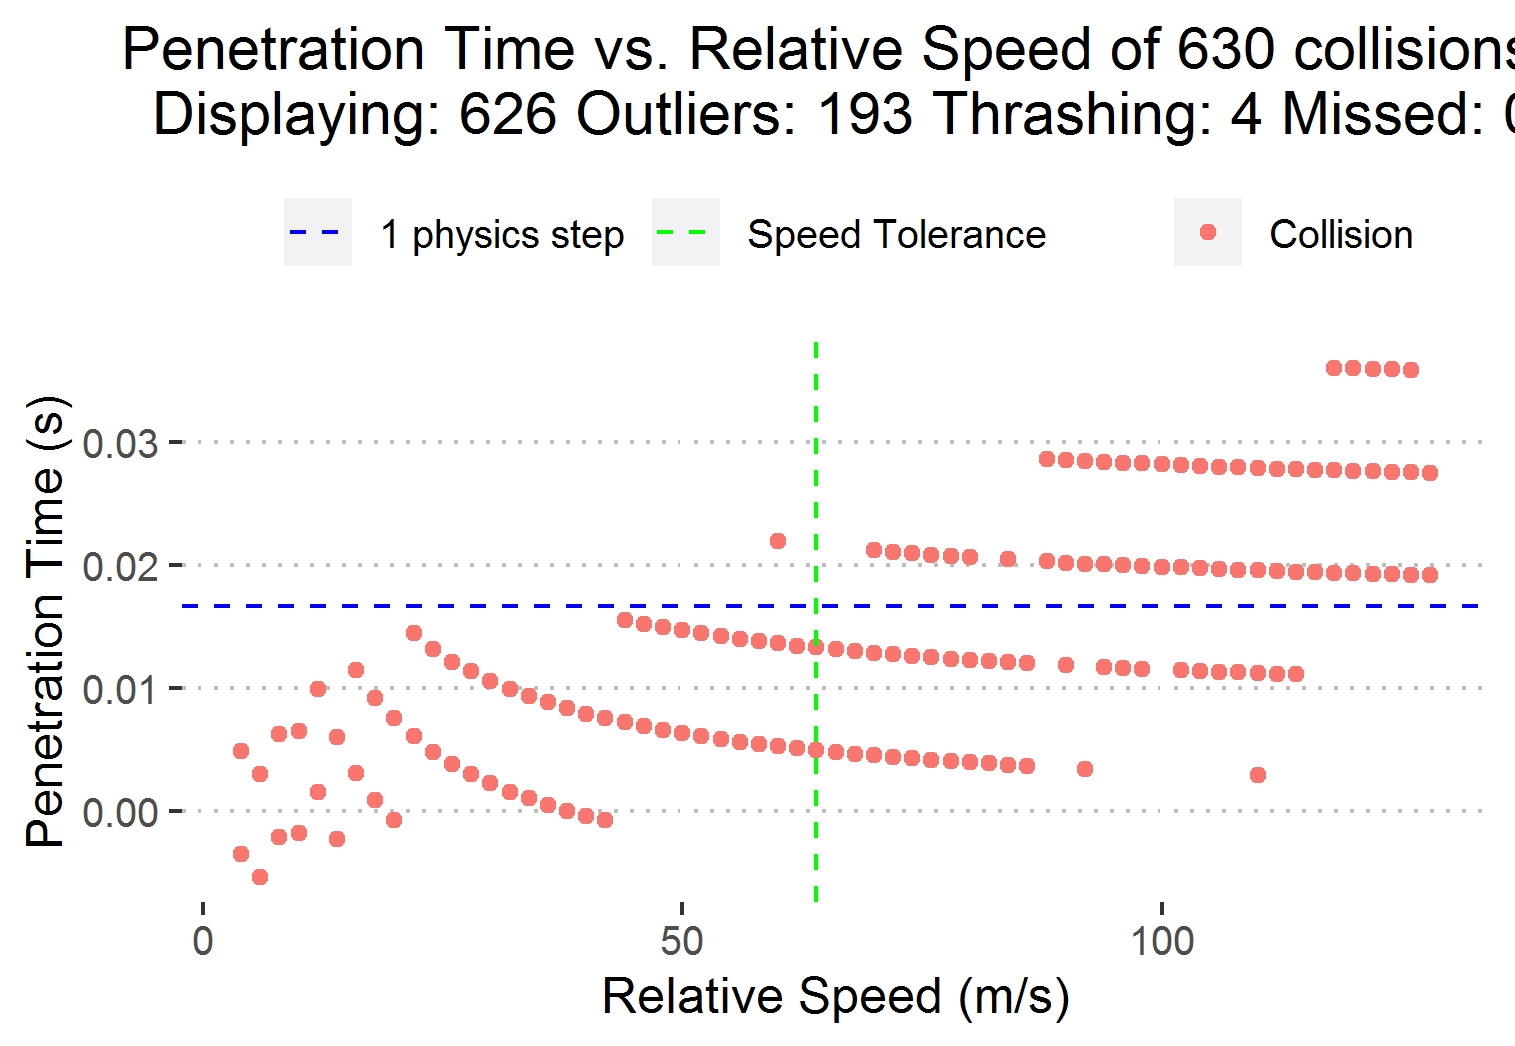
\includegraphics[width=\textwidth]{CollisionsPenVsSpeed}
	\caption{Penetration time of objects with varying relative speed. Each red point represents one or more collisions. The maximum expected penetration time of 1 physics steps is marked with a dashed blue line. The speed tolerance is marked in a dashed green line. The number and magnitude of errors increases as relative speed increases beyond the tolerance.}
	\label{fig_CollisionsPenVsSpeed}
\end{figure}

\begin{figure}
\centering
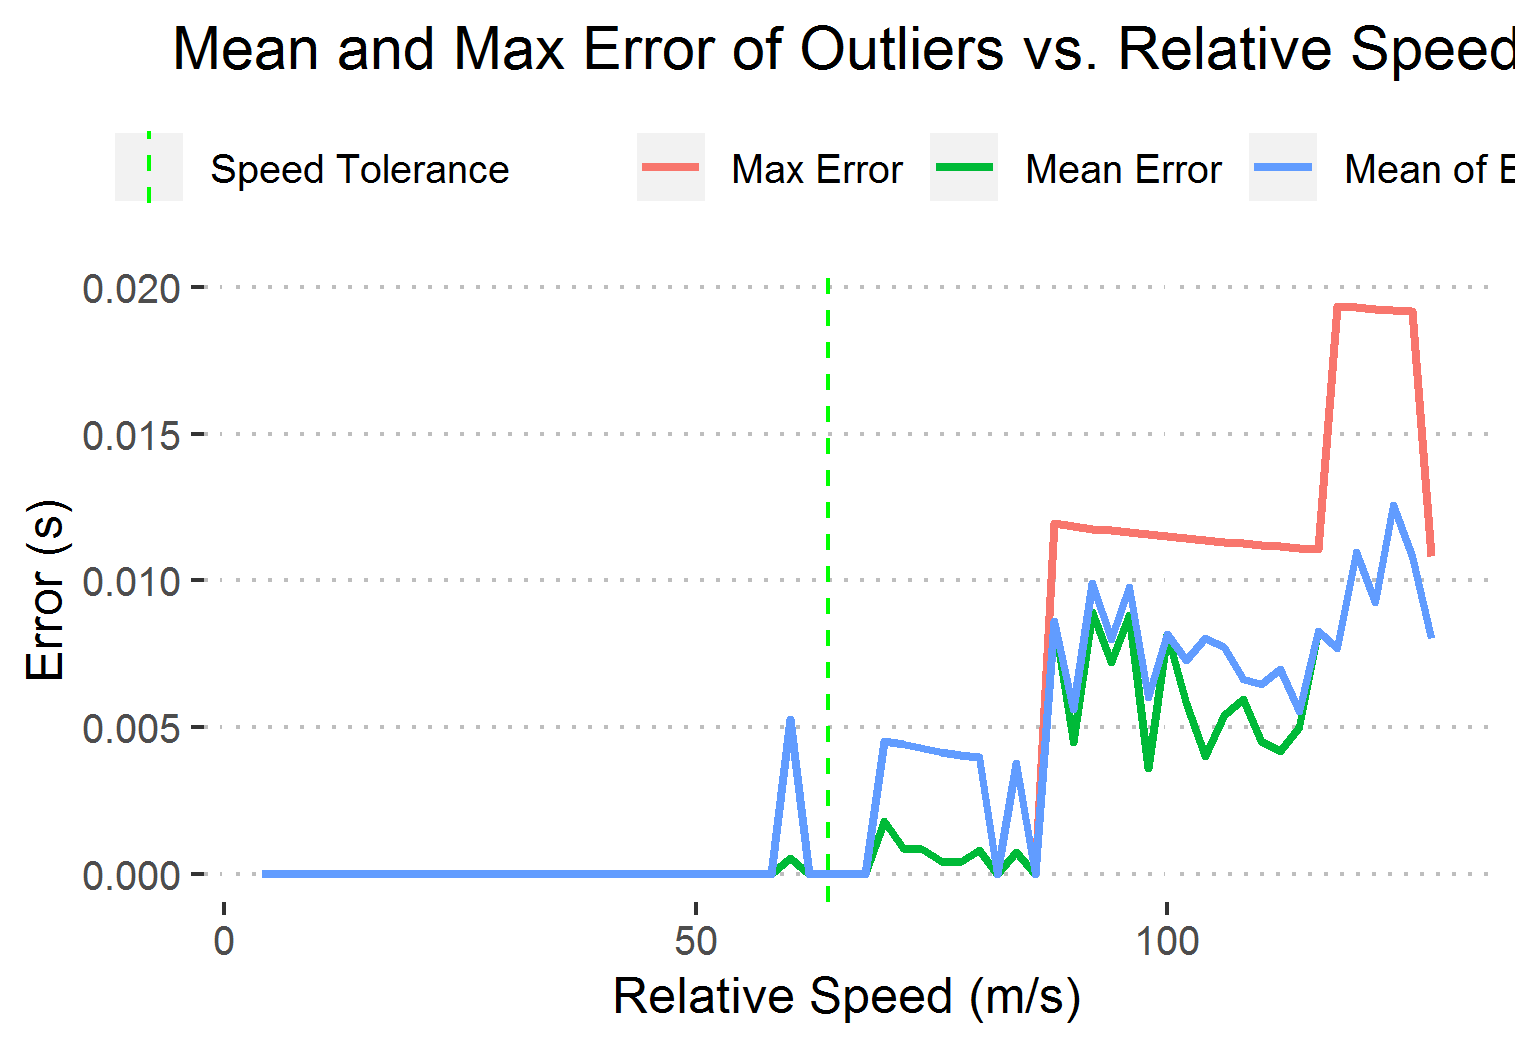
\includegraphics[width=\textwidth]{MeanMaxErrorVsSpeed}
\caption{The mean and max of collision errors with varying relative speed}
\label{fig_MeanMaxErrorVsSpeed}
\end{figure}

\begin{figure}
\centering
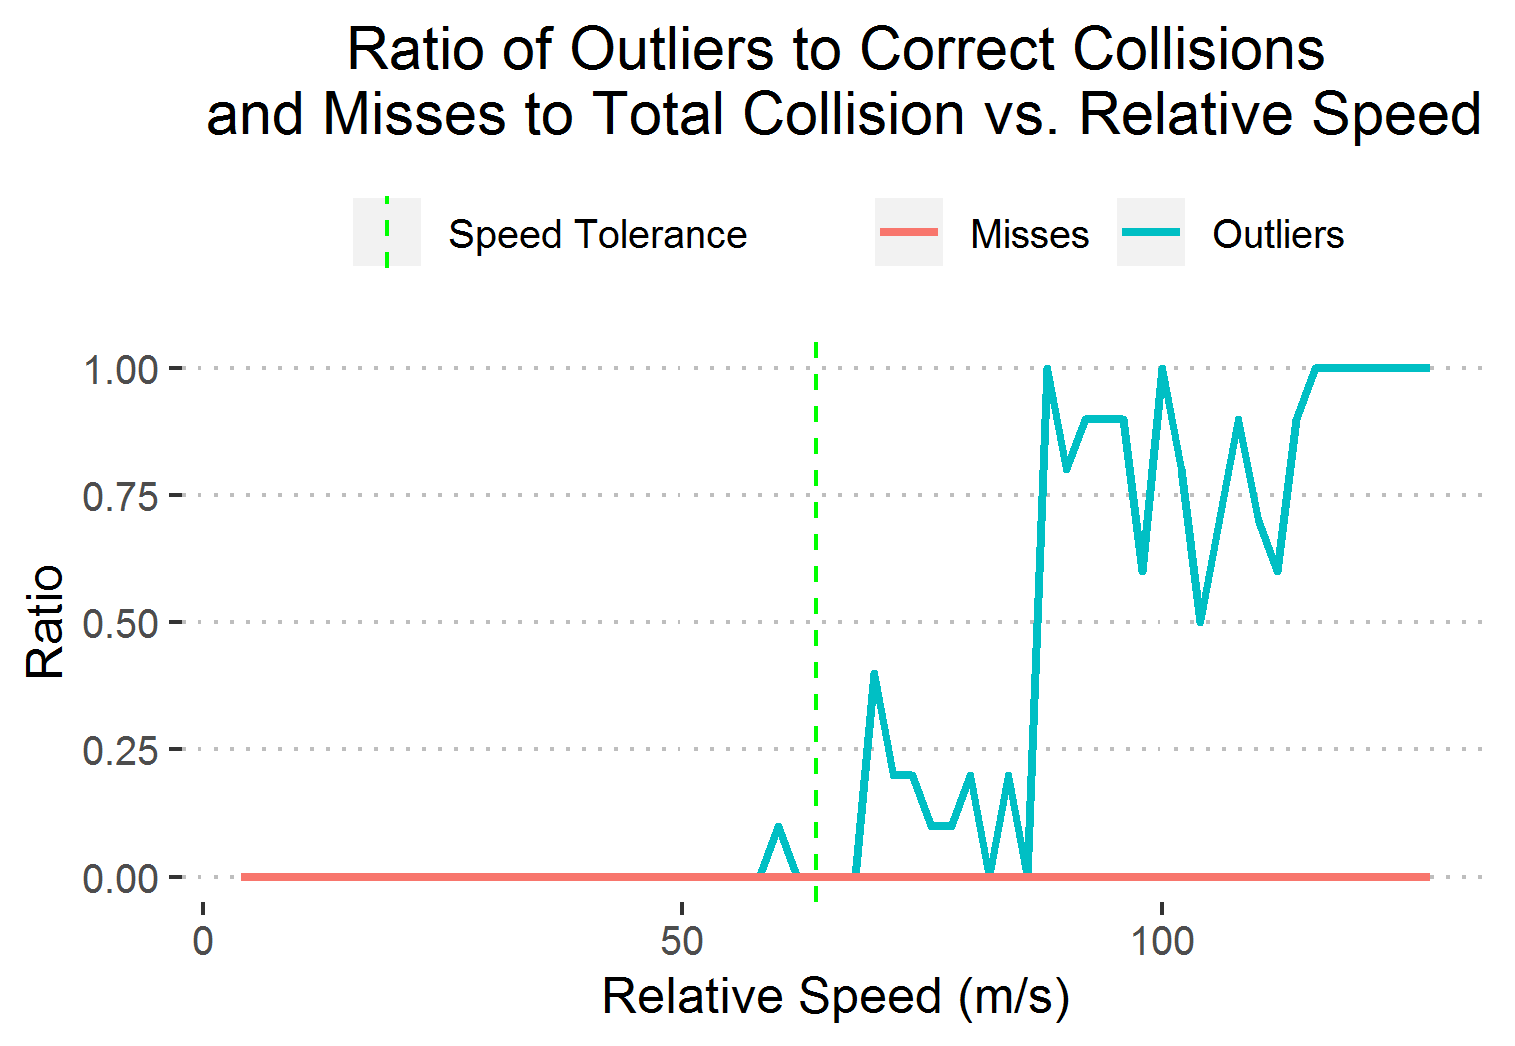
\includegraphics[width=\textwidth]{RatiosVsSpeed}
\caption{The ratios of erroneous collisions to correct collisions and missed collisions to total collisions with varying relative speed}
\label{fig_RatiosVsSpeed}
\end{figure}

\subsubsection{Varying Latency}

In this experiment the latency between the two servers was varied from $0ms$ to $40ms$ ($20*latency tolerance$) in increments of $1ms$. A high maximum factor of 20 was chosen as error increases slowly relative to the tolerance value. The latency used is the target latency, in reality the latency will never exactly be equal to $0ms$.

\begin{figure}
\centering
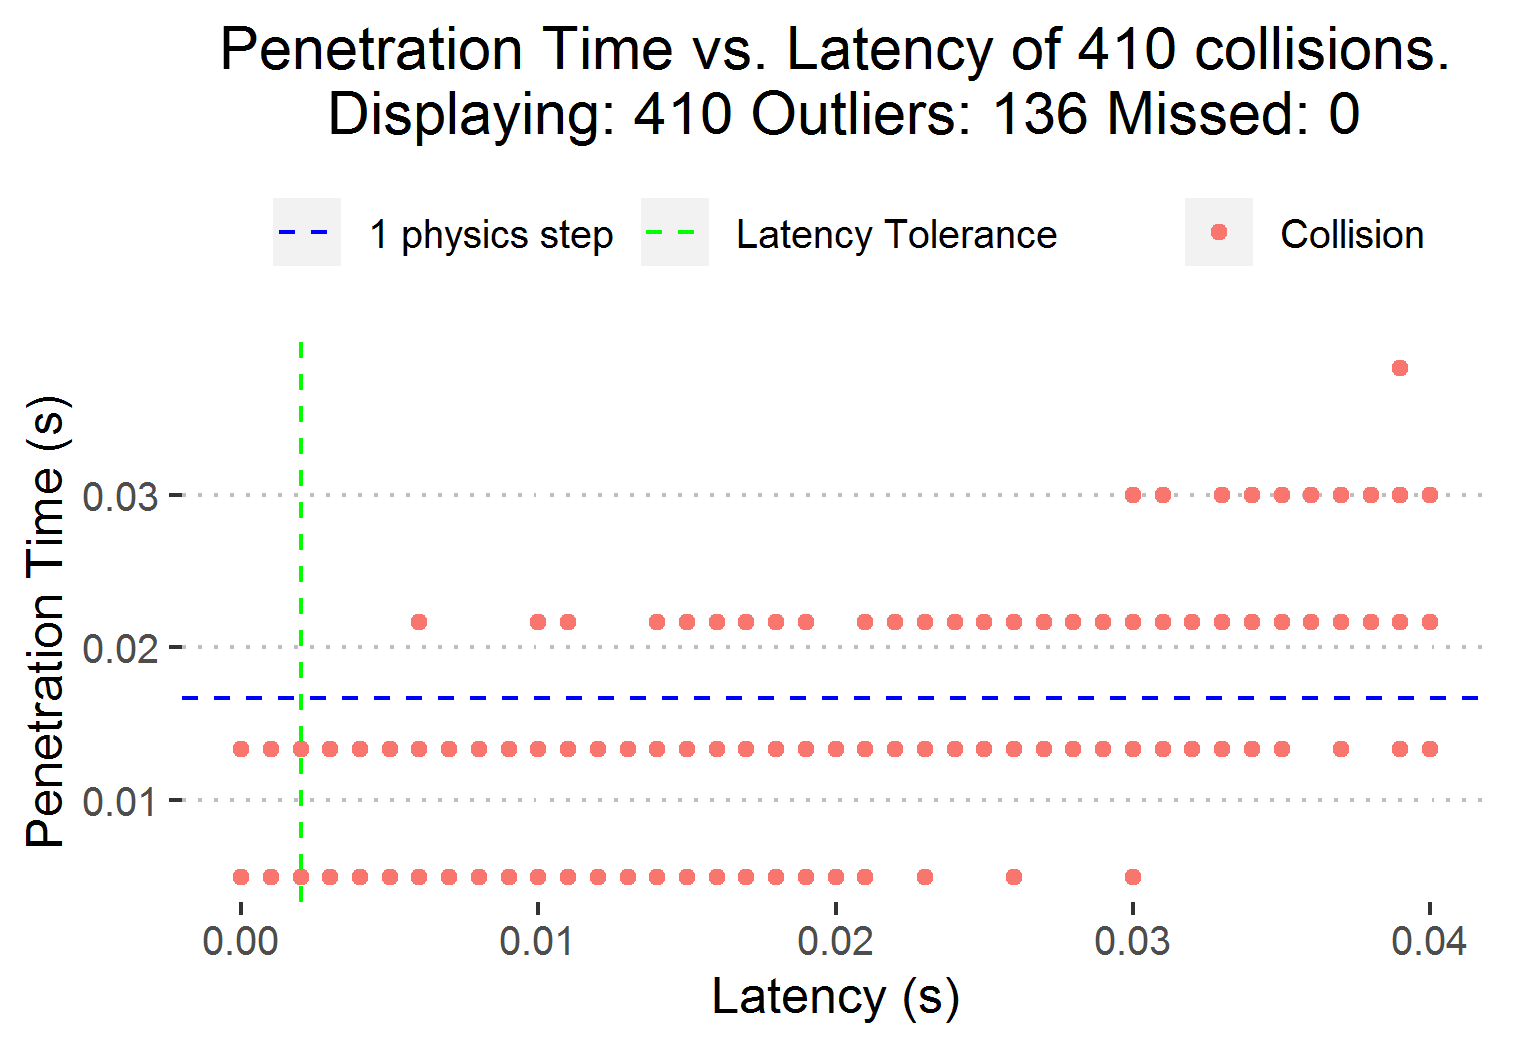
\includegraphics[width=\textwidth]{CollisionsPenVsLatency}
\caption{Penetration time of objects with varying latency. Each red point represents one or more collisions. The maximum expected penetration time of 1 physics steps is marked with a dashed blue line. The latency tolerance is marked in a dashed green line. The number and magnitude of errors increases as latency increases beyond the tolerance.}
\label{fig_CollisionsPenVsLatency}
\end{figure}

\begin{figure}
\centering
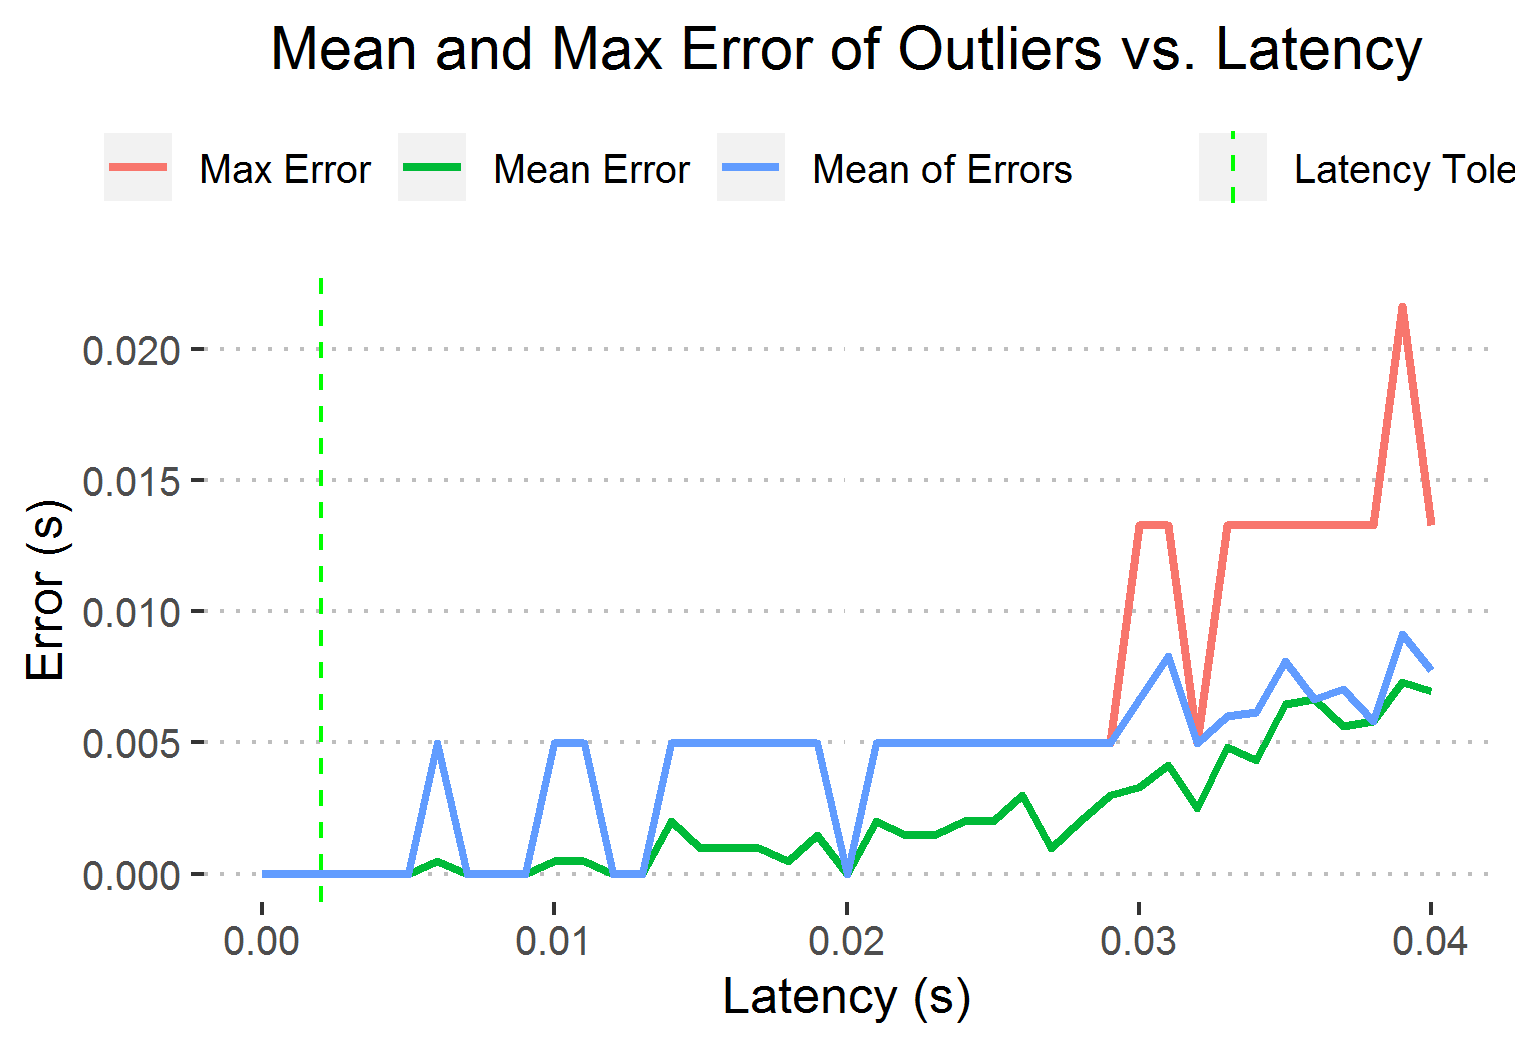
\includegraphics[width=\textwidth]{MeanMaxErrorVsLatency}
\caption{The mean and max of collision errors with varying latency}
\label{fig_MeanMaxErrorVsLatency}
\end{figure}

\begin{figure}
\centering
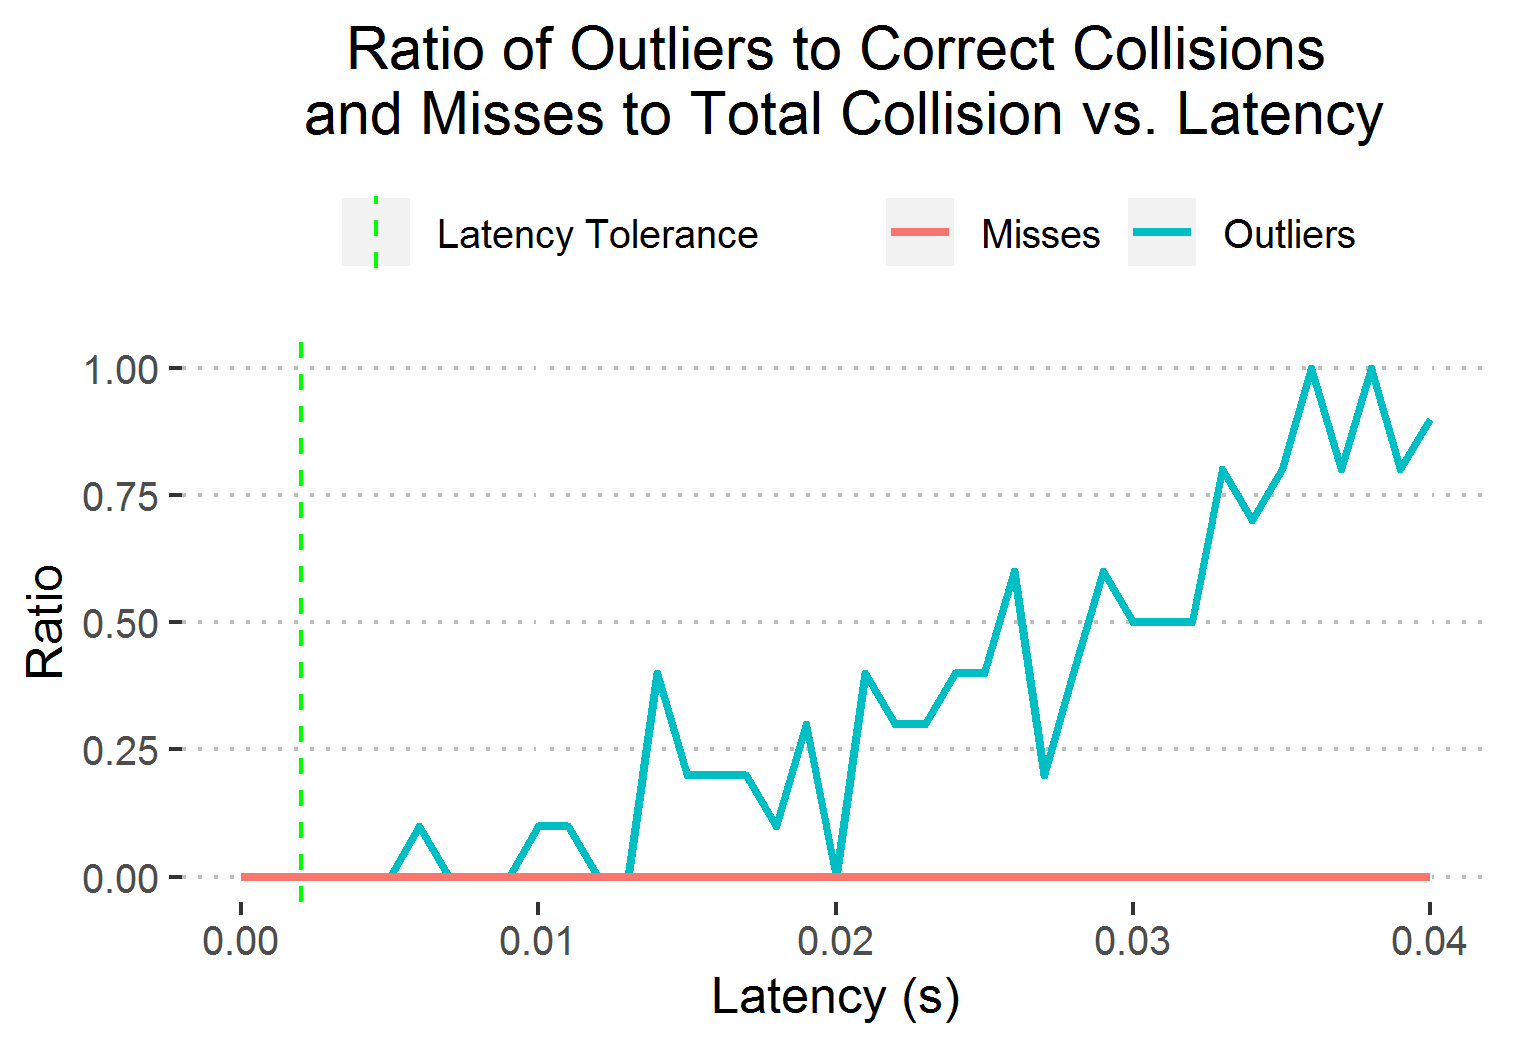
\includegraphics[width=\textwidth]{RatiosVsLatency}
\caption{The ratios of erroneous collisions to correct collisions and missed collisions to total collisions with varying latency}
\label{fig_RatiosVsLatency}
\end{figure}

\subsubsection{Varying Frame-Time}

In this experiment the frame-time was varied from $0ms$ to $30ms$ (double the frame-time tolerance) in increments of $1ms$.
The frame-time used is target frame time, in reality frame-time cannot be equal to exactly $0ms$

\begin{figure}
\centering
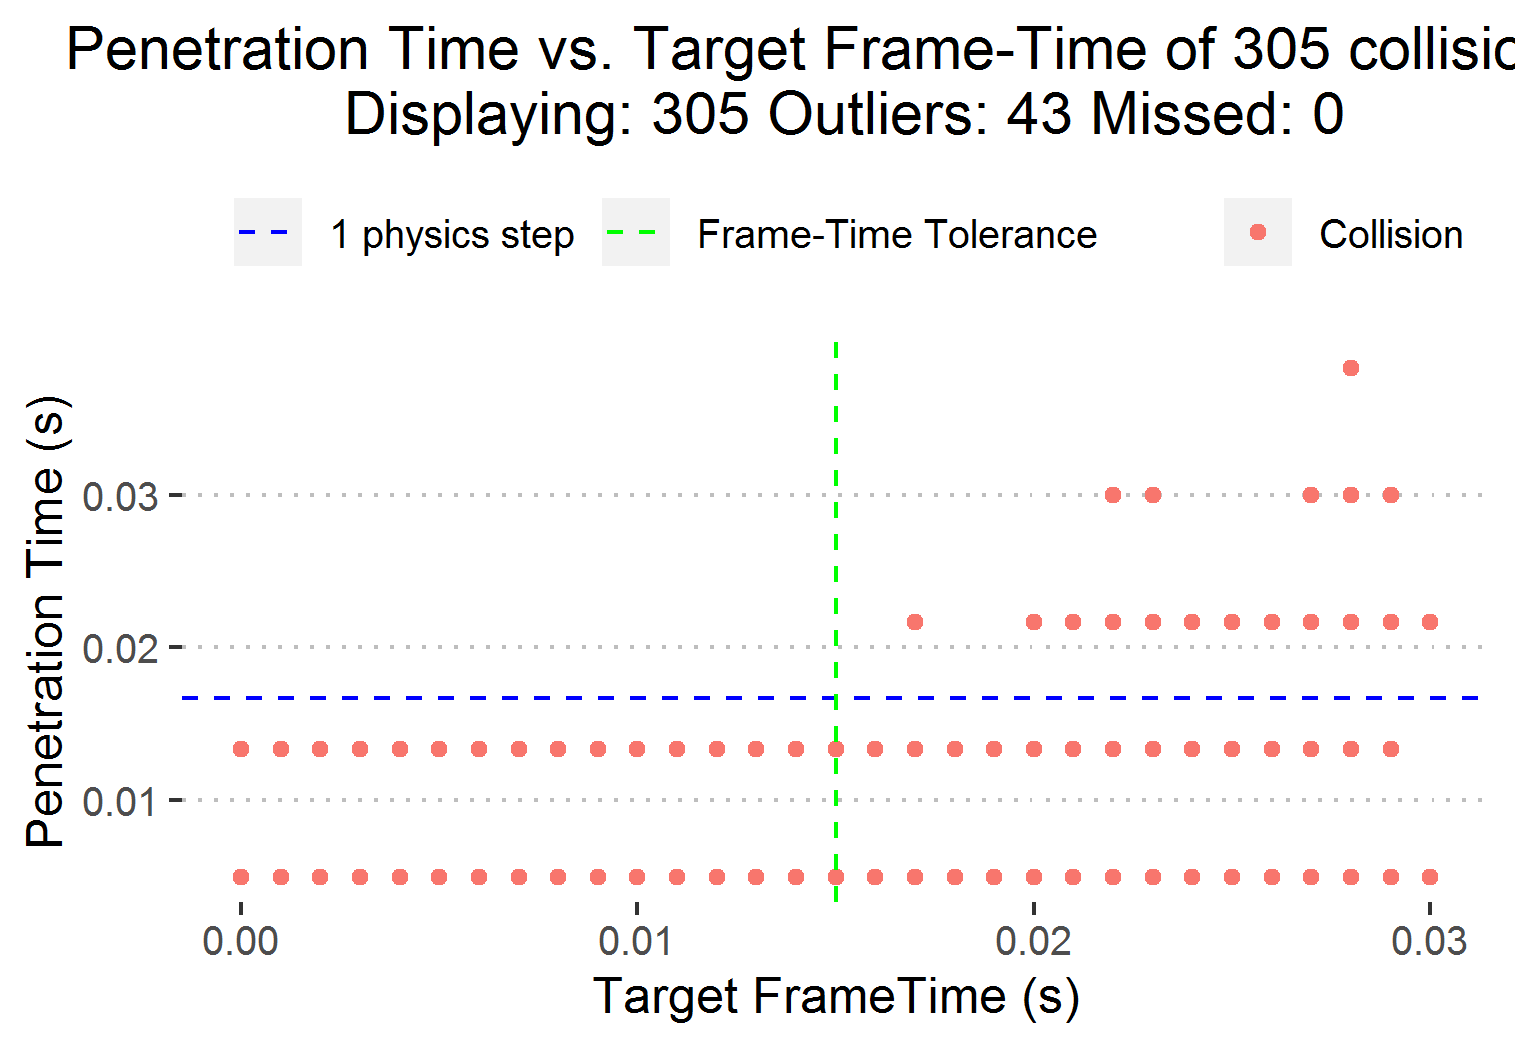
\includegraphics[width=\textwidth]{CollisionsPenVsFrameTime}
\caption{Penetration time of objects with varying frame-time. Each red point represents one or more collisions. The maximum expected penetration time of 1 physics steps is marked with a dashed blue line. The speed tolerance is marked in a dashed green line. The number and magnitude of errors increases as target frame-time increases beyond the tolerance.}
\label{fig_CollisionsPenVsFrameTime}
\end{figure}

\begin{figure}
\centering
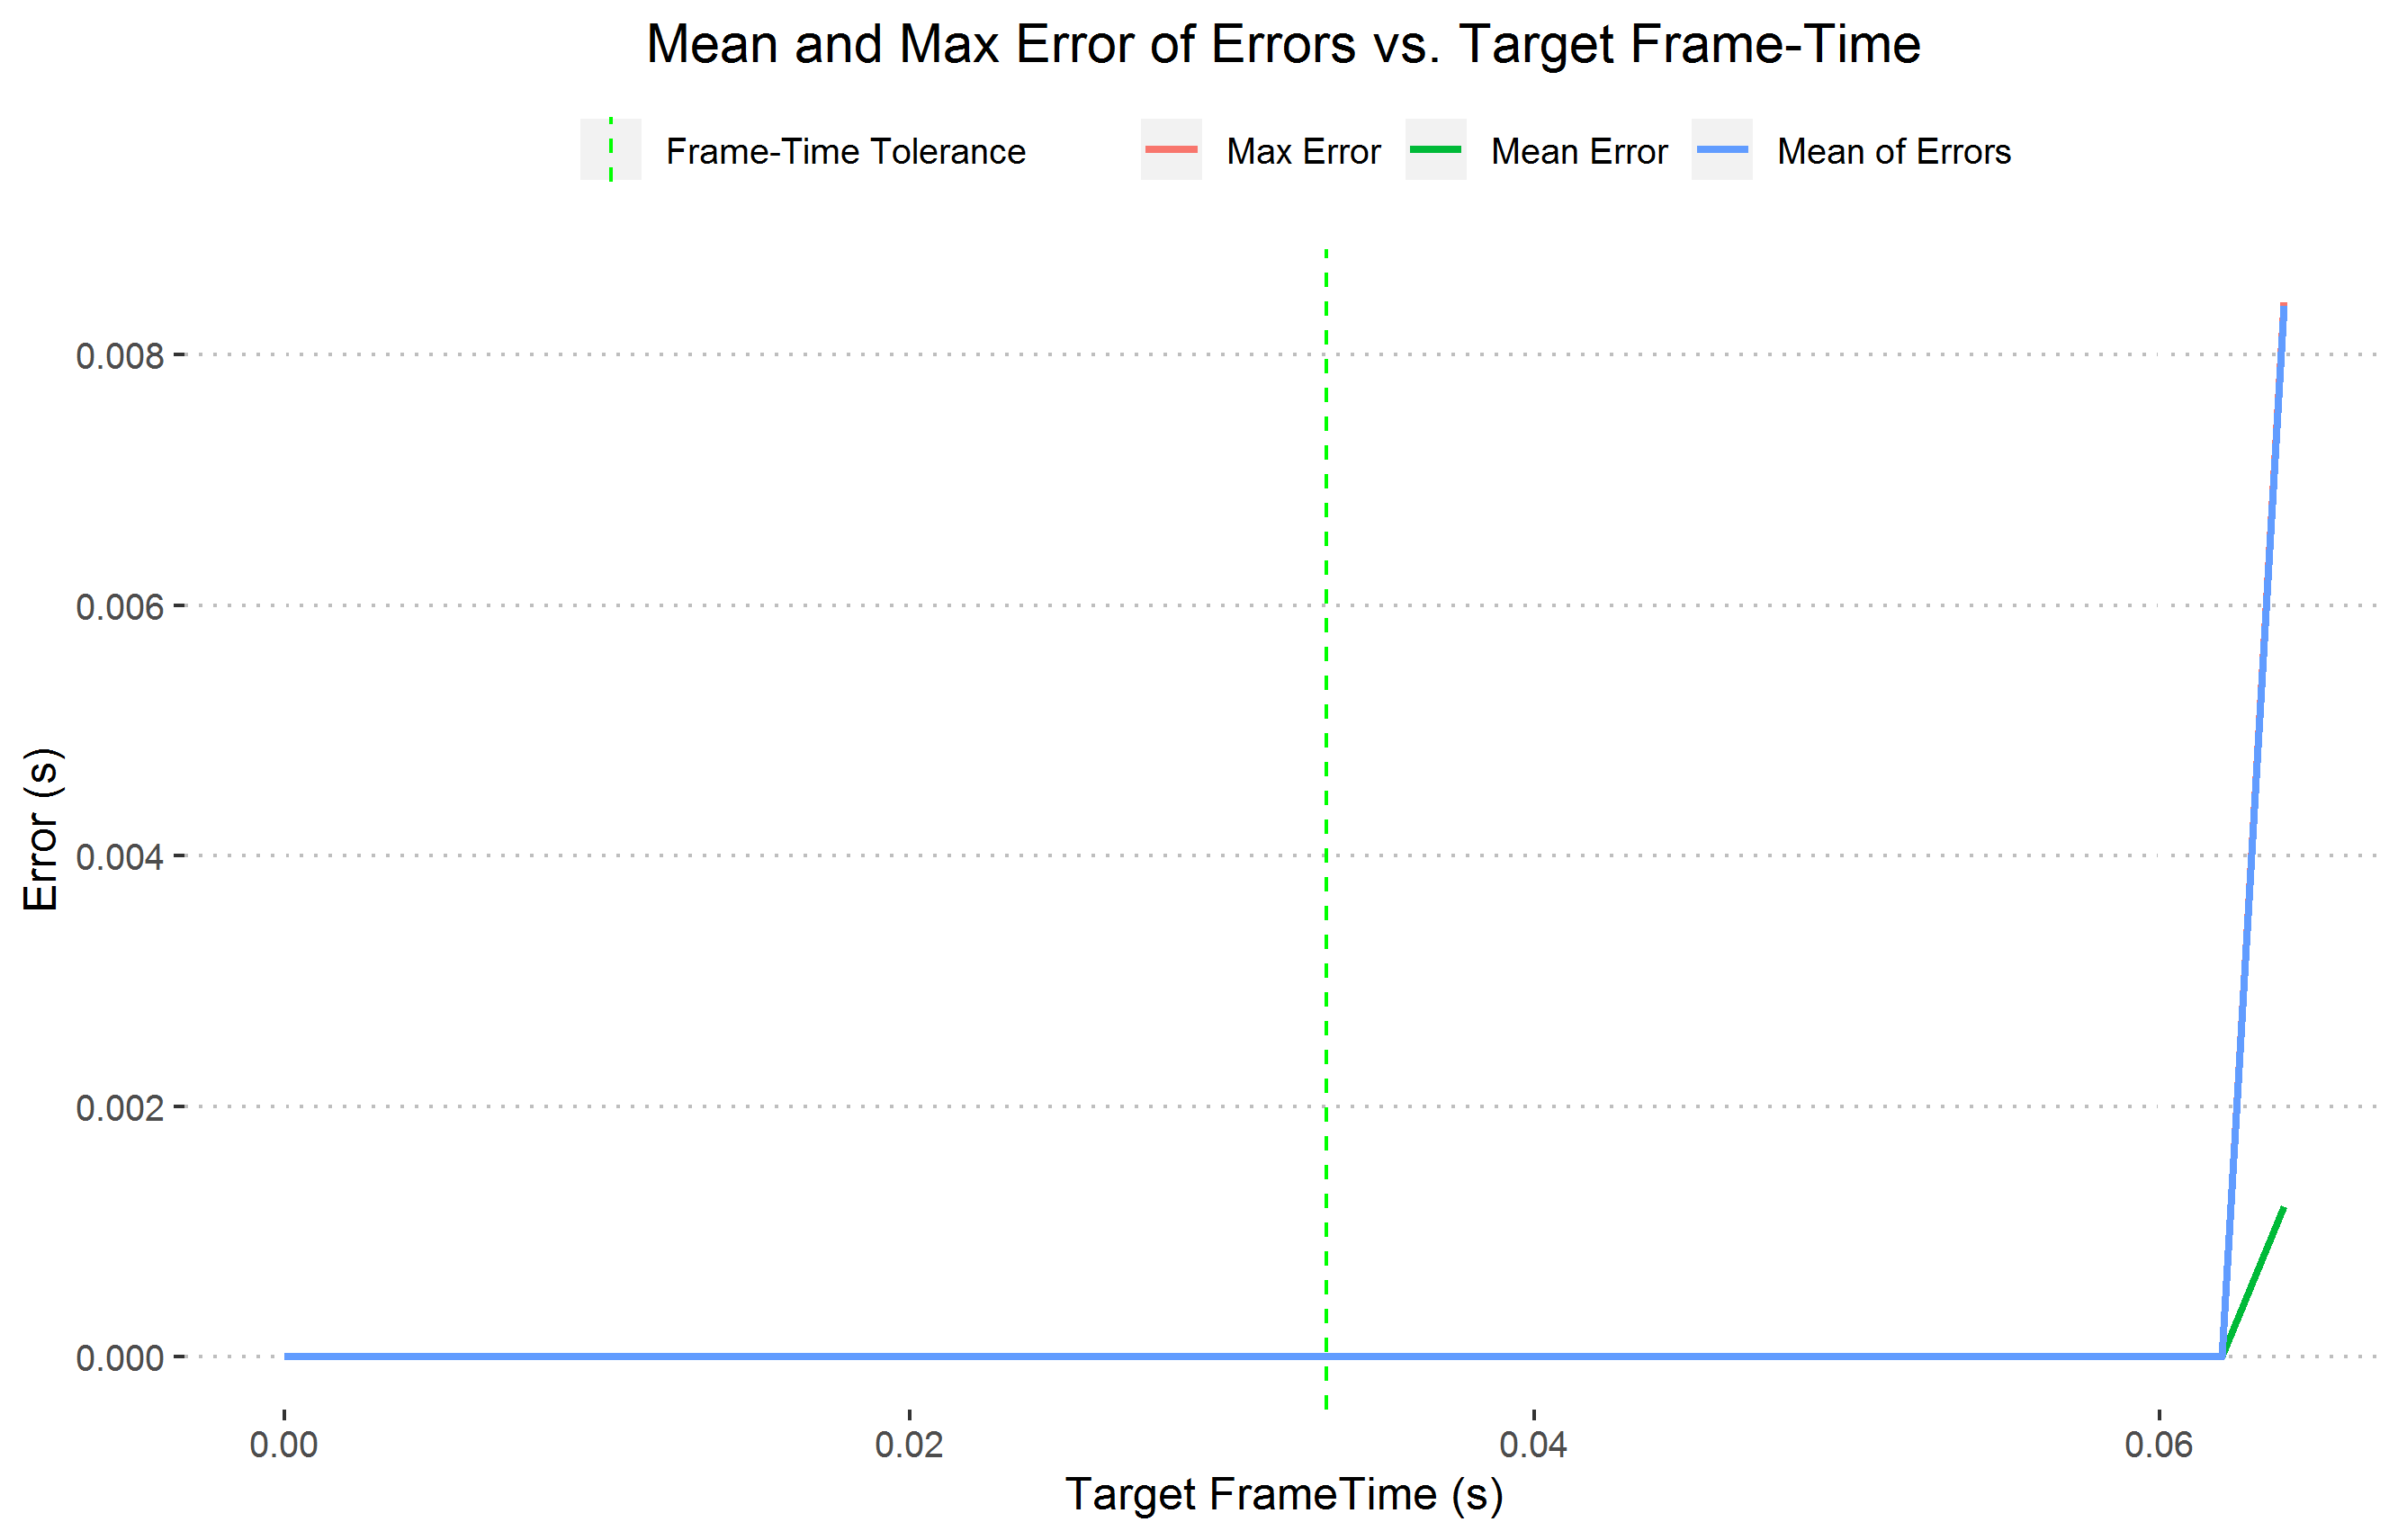
\includegraphics[width=\textwidth]{MeanMaxErrorVsFrameTime}
\caption{The mean and max of collision errors with varying frame-time}
\label{fig_MeanMaxErrorVsFrameTime}
\end{figure}

\begin{figure}
\centering
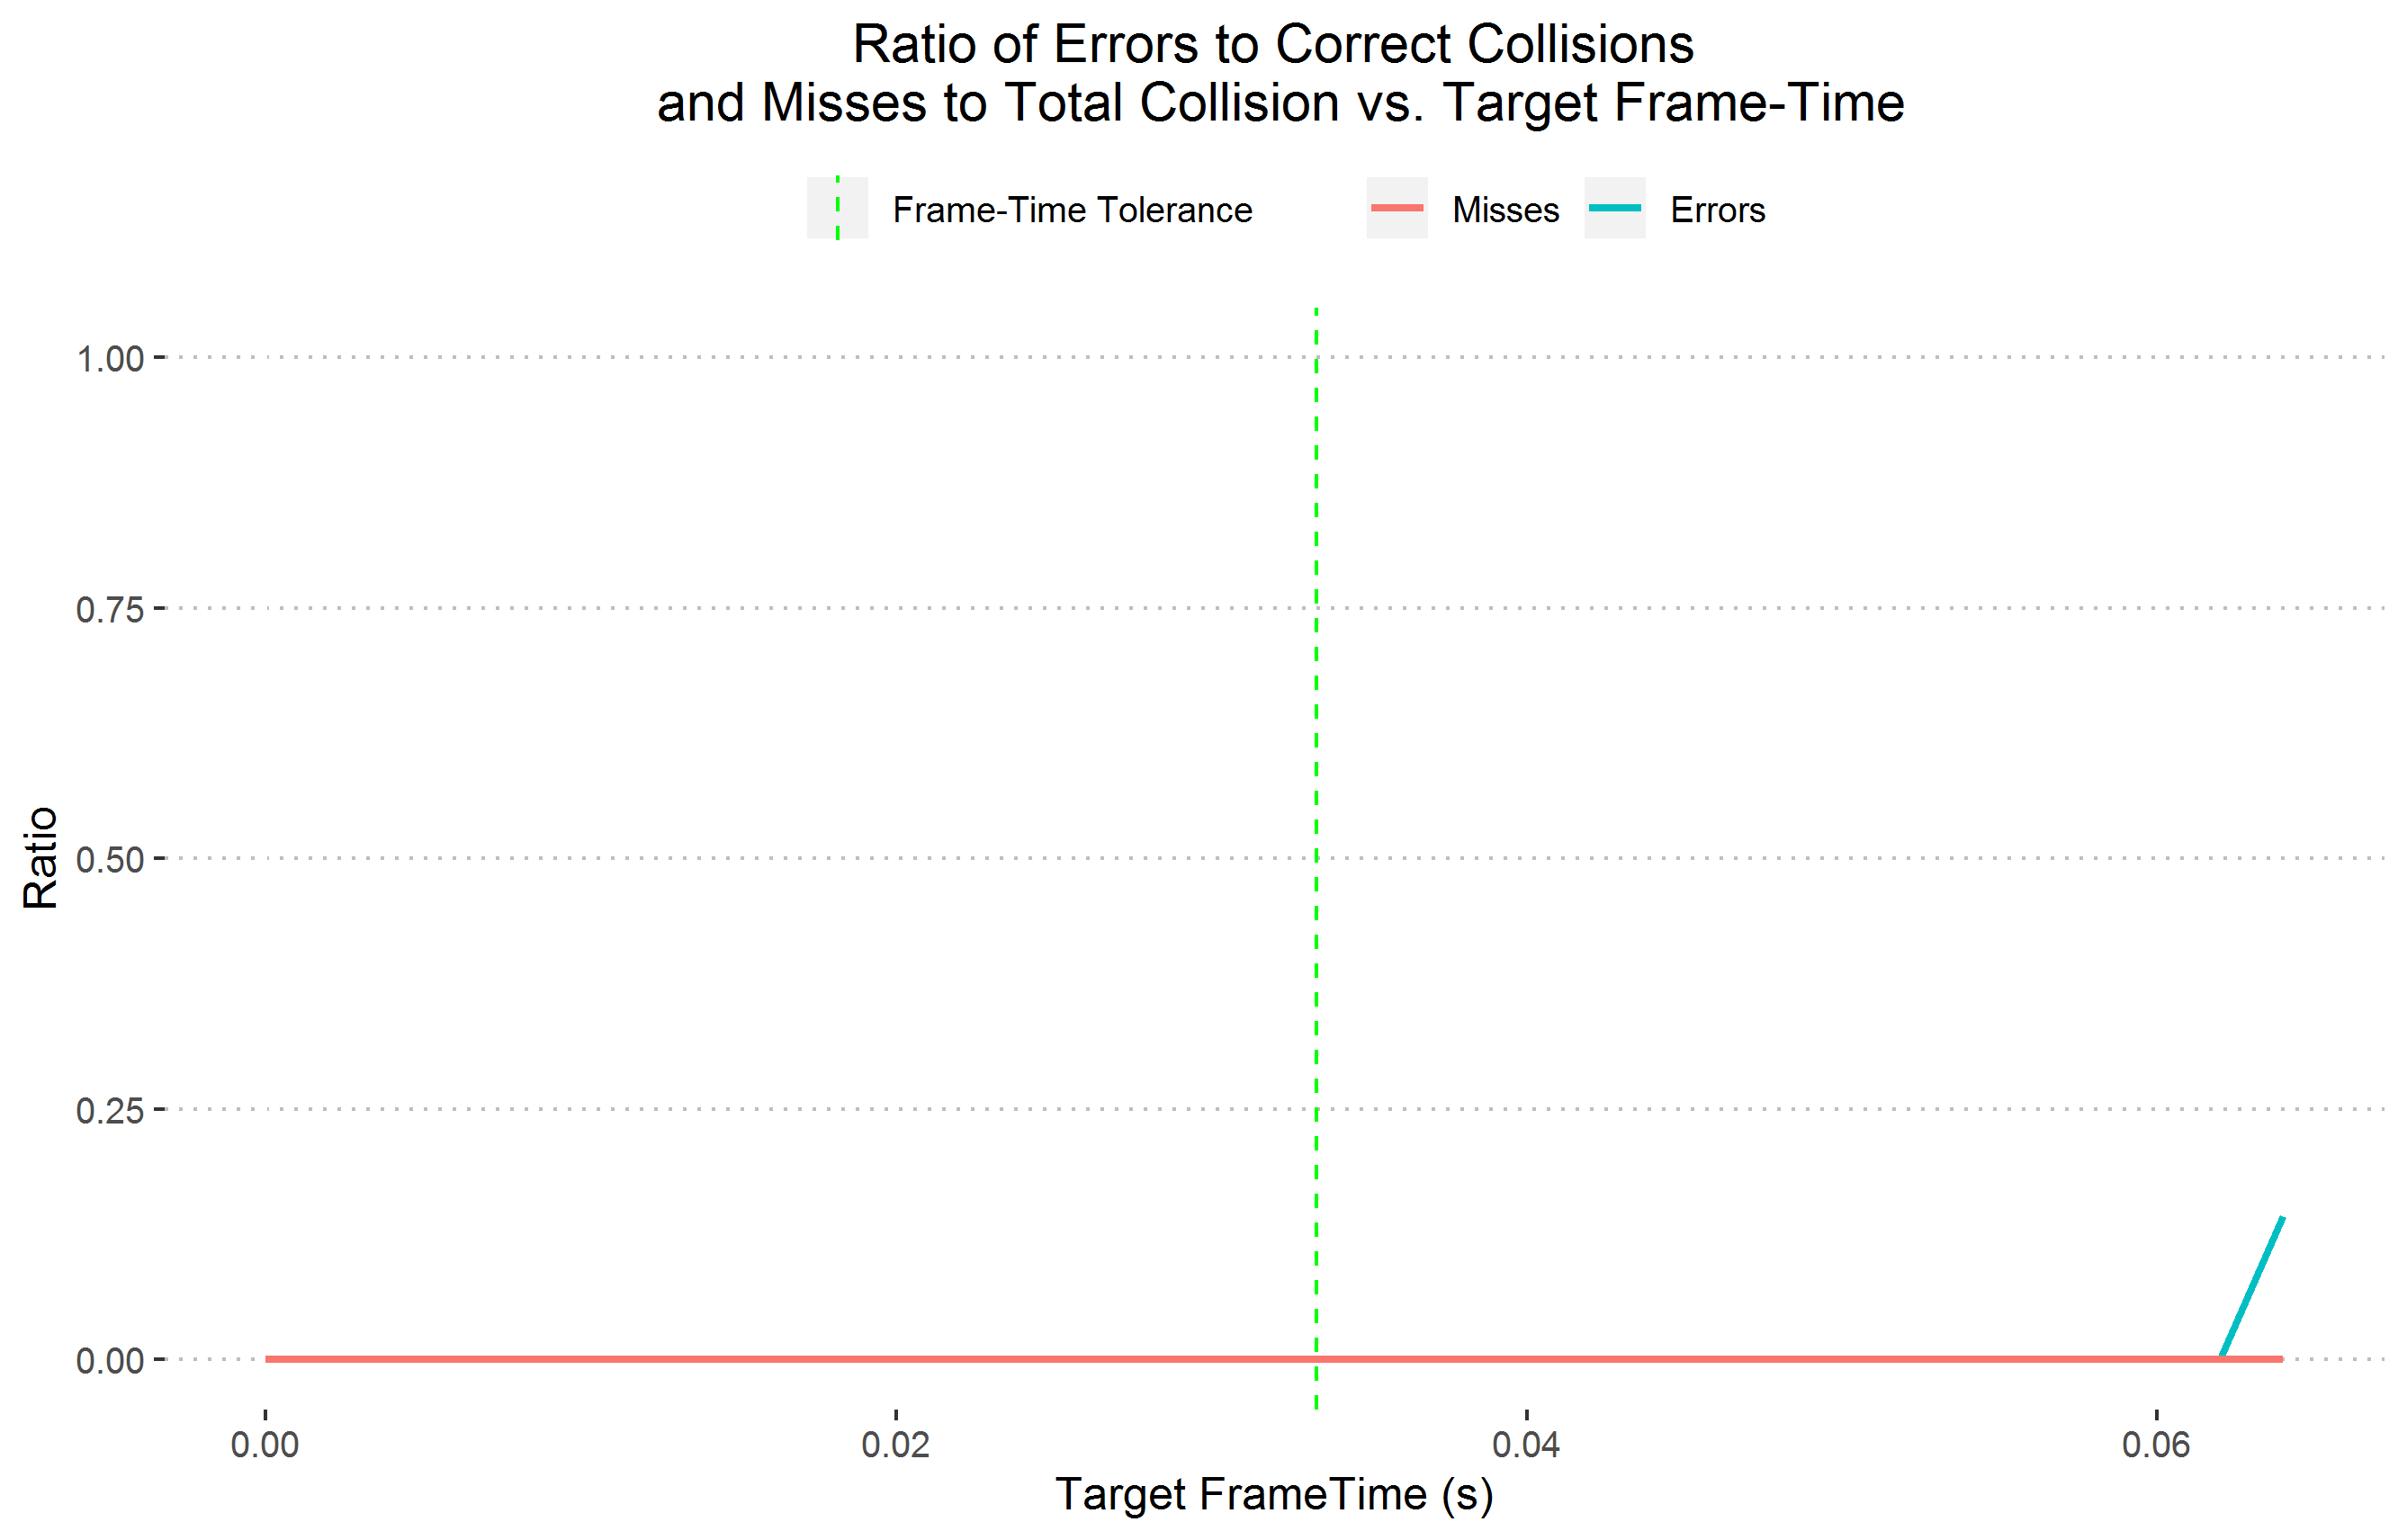
\includegraphics[width=\textwidth]{RatiosVsFrameTime}
\caption{The ratios of erroneous collisions to correct collisions and missed collisions to total collisions with varying frame-time}
\label{fig_RatiosVsFrameTime}
\end{figure}

\subsubsection{Evaluation}
The varying factors experiments demonstrate that the aura calculation is either correct or close to correct for all aura tolerance factors. For each varied factor below the tolerance value there are only a small number of erroneous collisions just below the tolerance value and no missed collisions. Once factors increase above the tolerance value erroneous collisions begin to occur with increasing number and magnitude.

%TODO: Talk about how errors increase with each factor
%TODO: Check for small numbers of errors below tolerances
%There are no erroneous collisions below the tolerance apart from in the latency experiment, but I was expecting a small number of errors below the tolerance lines due to the way the frame-time control works

\subsection{Varying Packet-Loss}

In addition to varying each aura tolerance factor, an experiment was also carried out to determine the effects of packet-loss on the correctness of collisions between objects. In this experiment the packet-loss was varied from $0\%$ to $80\%$ in increments of $10\%$. Packet-loss is not factored into the aura calculation and therefore has no tolerance. Packet-loss is controlled using the Traffic Manager tool; packet-loss is emulated on each server for all communication received from the other server.

RakNet, the library used for network communication in this project, includes a reliability layer. This means if packets are lost and an acknowledgement message is not received, sending will be re-attempted. However, this takes time and therefore causes a delay in messages being received. Delays in messages will lead to erroneous collisions, therefore as packet-loss increases, erroneous collisions should increase in number and magnitude. If messages are delayed enough, the collision will be missed as the two objects pass each other on different servers without ever interacting with each other. 

%TODO: Check if aura updates are ordered, mention that here.
%RakNet's reliability layer uses best effort, meaning messages are not guaranteed to be received, which means some messages may never be received resulting in 

\begin{figure}
\centering
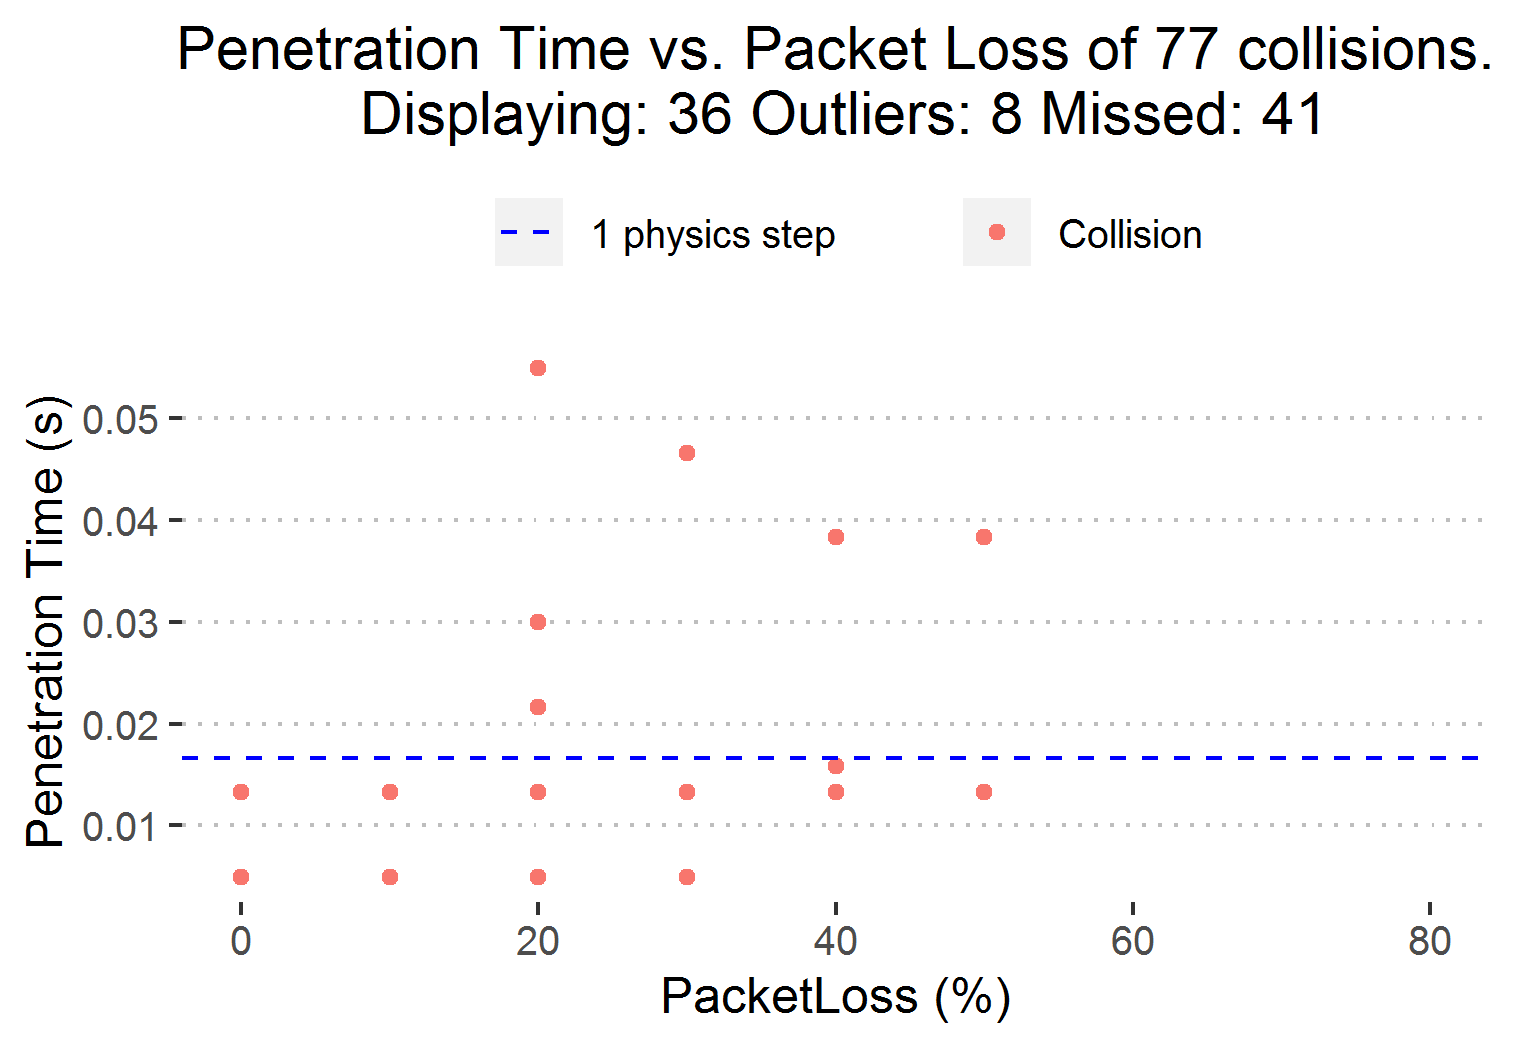
\includegraphics[width=\textwidth]{CollisionsPenVsLoss}
\caption{Penetration time of objects with varying packet-loss. Each red point represents one or more collisions. The maximum expected penetration time of 1 physics steps is marked with a dashed blue line. The number and magnitude of errors increases as packet-loss increases beyond $10\%$.}
\label{fig_CollisionsPenVsLoss}
\end{figure}

\begin{figure}
\centering
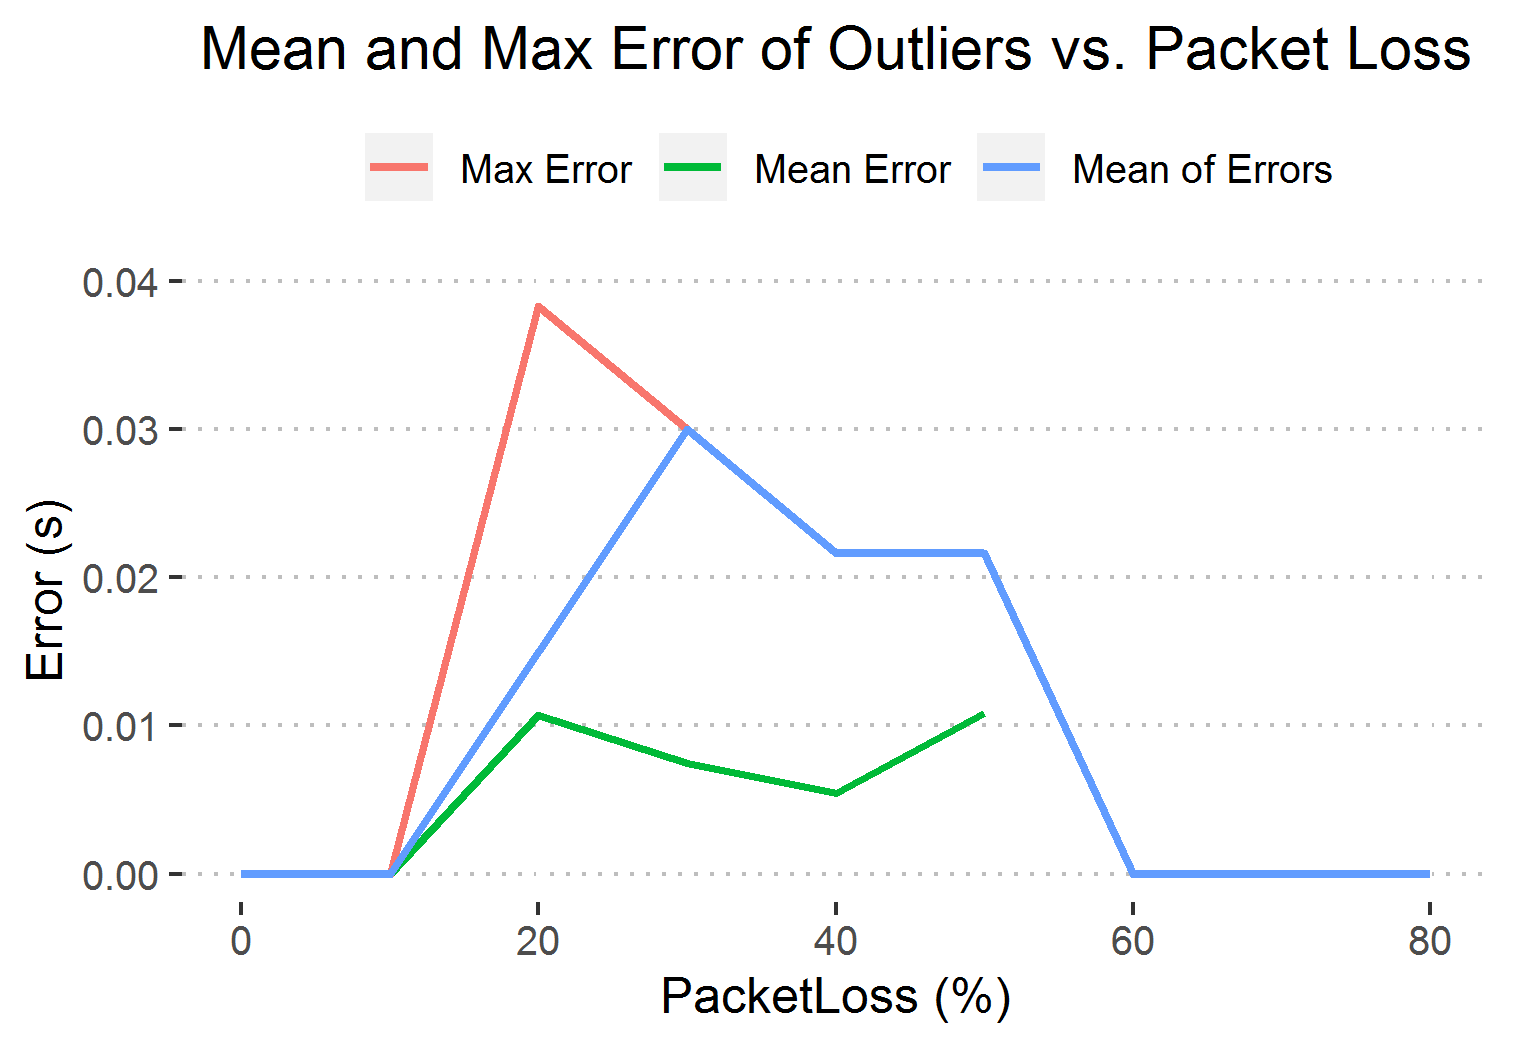
\includegraphics[width=\textwidth]{MeanMaxErrorVsLoss}
\caption{The mean and max of collision errors with varying packet loss. As packet-loss increases from $10\%$ to $20\%$ the magnitude of errors sharply increases until above $60\%$ where all collisions are missed so there is no error.}
\label{fig_MeanMaxErrorVsLoss}
\end{figure}

\begin{figure}
\centering
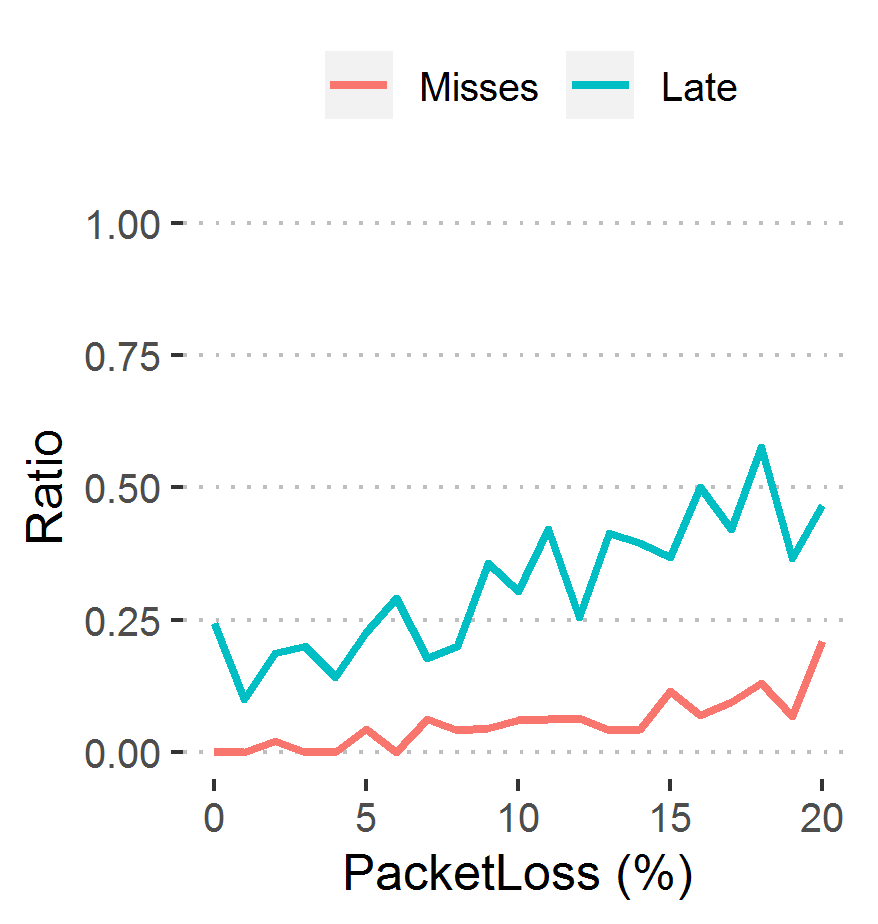
\includegraphics[width=\textwidth]{RatiosVsLoss}
\caption{The ratios of erroneous collisions to correct collisions and missed collisions to total collisions with varying packet loss. As packet-loss increases from $10\%$ to $20\%$ the ratio of erroneous collisions to correct collisions sharply increases as does misses to total collisions. Above $60\%$ packet-loss, all collisions are missed.}
\label{fig_RatiosVsLoss}
\end{figure}

\subsubsection{Evaluation}

\section{Communication Correctness Experiments}
%Will look for missing/duplicate objects auras. Dangling auras

\section{Case Study: Suspension Bridge}
